\documentclass[10pt,letterpaper]{article}\usepackage[]{graphicx}\usepackage[]{color}
%% maxwidth is the original width if it is less than linewidth
%% otherwise use linewidth (to make sure the graphics do not exceed the margin)
\makeatletter
\def\maxwidth{ %
  \ifdim\Gin@nat@width>\linewidth
    \linewidth
  \else
    \Gin@nat@width
  \fi
}
\makeatother

\definecolor{fgcolor}{rgb}{0.345, 0.345, 0.345}
\newcommand{\hlnum}[1]{\textcolor[rgb]{0.686,0.059,0.569}{#1}}%
\newcommand{\hlstr}[1]{\textcolor[rgb]{0.192,0.494,0.8}{#1}}%
\newcommand{\hlcom}[1]{\textcolor[rgb]{0.678,0.584,0.686}{\textit{#1}}}%
\newcommand{\hlopt}[1]{\textcolor[rgb]{0,0,0}{#1}}%
\newcommand{\hlstd}[1]{\textcolor[rgb]{0.345,0.345,0.345}{#1}}%
\newcommand{\hlkwa}[1]{\textcolor[rgb]{0.161,0.373,0.58}{\textbf{#1}}}%
\newcommand{\hlkwb}[1]{\textcolor[rgb]{0.69,0.353,0.396}{#1}}%
\newcommand{\hlkwc}[1]{\textcolor[rgb]{0.333,0.667,0.333}{#1}}%
\newcommand{\hlkwd}[1]{\textcolor[rgb]{0.737,0.353,0.396}{\textbf{#1}}}%
\let\hlipl\hlkwb

\usepackage{framed}
\makeatletter
\newenvironment{kframe}{%
 \def\at@end@of@kframe{}%
 \ifinner\ifhmode%
  \def\at@end@of@kframe{\end{minipage}}%
  \begin{minipage}{\columnwidth}%
 \fi\fi%
 \def\FrameCommand##1{\hskip\@totalleftmargin \hskip-\fboxsep
 \colorbox{shadecolor}{##1}\hskip-\fboxsep
     % There is no \\@totalrightmargin, so:
     \hskip-\linewidth \hskip-\@totalleftmargin \hskip\columnwidth}%
 \MakeFramed {\advance\hsize-\width
   \@totalleftmargin\z@ \linewidth\hsize
   \@setminipage}}%
 {\par\unskip\endMakeFramed%
 \at@end@of@kframe}
\makeatother

\definecolor{shadecolor}{rgb}{.97, .97, .97}
\definecolor{messagecolor}{rgb}{0, 0, 0}
\definecolor{warningcolor}{rgb}{1, 0, 1}
\definecolor{errorcolor}{rgb}{1, 0, 0}
\newenvironment{knitrout}{}{} % an empty environment to be redefined in TeX

\usepackage{alltt}
\usepackage[top=0.85in,left=1.75in,footskip=0.75in]{geometry}

% amsmath and amssymb packages, useful for mathematical formulas and symbols
\usepackage{amsmath,amssymb}

% Use adjustwidth environment to exceed column width (see example table in text)
\usepackage{changepage}

% Use Unicode characters when possible
\usepackage[utf8x]{inputenc}

% textcomp package and marvosym package for additional characters
\usepackage{textcomp,marvosym}

% cite package, to clean up citations in the main text. Do not remove.
\usepackage{cite}

% Use nameref to cite supporting information files (see Supporting Information section for more info)
\usepackage{nameref,hyperref}

% line numbers
\usepackage[right]{lineno}

% ligatures disabled
\usepackage{microtype}
\DisableLigatures[f]{encoding = *, family = * }

% color can be used to apply background shading to table cells only
\usepackage[table]{xcolor}

% array package and thick rules for tables
\usepackage{array}

% bold math symbols package
\usepackage{bm}

% nice figures and captions
\usepackage{graphicx}

%\usepackage{floatflt}
%\usepackage{nonfloat}
\usepackage{float}
\usepackage{wrapfig}

%\renewcommand{\arraystretch}{1.2}
%\setlength{\tabcolsep}{12pt}

% create "+" rule type for thick vertical lines
\newcolumntype{+}{!{\vrule width 2pt}}

% create \thickcline for thick horizontal lines of variable length
\newlength\savedwidth
\newcommand\thickcline[1]{%
  \noalign{\global\savedwidth\arrayrulewidth\global\arrayrulewidth 2pt}%
  \cline{#1}%
  \noalign{\vskip\arrayrulewidth}%
  \noalign{\global\arrayrulewidth\savedwidth}%
}

% \thickhline command for thick horizontal lines that span the table
\newcommand\thickhline{\noalign{\global\savedwidth\arrayrulewidth\global\arrayrulewidth 2pt}%
\hline
\noalign{\global\arrayrulewidth\savedwidth}}


% Remove comment for double spacing
%\usepackage{setspace} 
%\doublespacing

% Text layout
% \raggedright
\setlength{\parindent}{0.5cm}
\textwidth 5.25in 
\textheight 8.75in

% Bold the 'Figure #' in the caption and separate it from the title/caption with a period
% Captions will be left justified
\usepackage[aboveskip=1pt,labelfont=bf,labelsep=period,justification=raggedright,singlelinecheck=off]{caption}
\renewcommand{\figurename}{Fig}

% Use the PLoS provided BiBTeX style
%\bibliographystyle{plos2015}


% Remove brackets from numbering in List of References
\makeatletter
\renewcommand{\@biblabel}[1]{\quad#1.}
\makeatother

% define theorem and definition environments commands
\newtheorem{theorem}{Theorem}[section]
\newtheorem{definition}{Definition}[section]

% Header and Footer with logo
\usepackage{lastpage,fancyhdr,graphicx}
\usepackage{epstopdf}
%\pagestyle{myheadings}
\pagestyle{fancy}
\fancyhf{}
%\setlength{\headheight}{27.023pt}
%\lhead{\includegraphics[width=2.0in]{PLOS-submission.eps}}
\rfoot{\thepage/\pageref{LastPage}}
\renewcommand{\headrulewidth}{0pt}
\renewcommand{\footrule}{\hrule height 2pt \vspace{2mm}}
\fancyheadoffset[L]{2.25in}
% \fancyfootoffset[L]{1.25in}
\lfoot{\today}


\restylefloat{figure}


%% Include all macros below

\newcommand{\lorem}{{\bf LOREM}}
\newcommand{\ipsum}{{\bf IPSUM}}

\def\lf{\left\lfloor}   
\def\rf{\right\rfloor}

\def\ri{R_i}
\def\rj{R_j}
\def\kmi{k_{M_i}}
\def\khi{k_{H_i}}
\def\hji{H_{j_i}}
\def\ma{\overline{M}_a}
\def\ha{\overline{H}_a}
\def\mnu{M_\nu}
\def\hnu{H_\nu}
\def\myd{\text{diff}}
\def\ka{\bar{k}_\alpha}
\def\mji{M_{j_i}}

%% END MACROS SECTION
\IfFileExists{upquote.sty}{\usepackage{upquote}}{}
\begin{document}
\vspace*{0.2in}

% Title must be 250 characters or less.
% \begin{flushleft}
{\Large
\textbf\newline{Blessings of Dimensionality: Theoretical analysis of nearest-neighbor projected-distance methods for detecting interactions in high dimensional data} % Please use "sentence case" for title and headings (capitalize only the first word in a title (or heading), the first word in a subtitle (or subheading), and any proper nouns).
}
%\newline
% Insert author names, affiliations and corresponding author email (do not include titles, positions, or degrees).
\begin{center}
  \begin{tabular}{l}
  Bryan A. Dawkins$^{\text{1}}$, Trang T. Le$^{\text{2}}$ and Brett A. McKinney$^{\text{1,3,}*}$ \\
  $^{\text{1}}$Department of Mathematics, University of Tulsa, Tulsa, OK 74104, USA \\
  $^{\text{2}}$Department of Biostatistics, Epidemiology and Informatics, University of \\
  \hphantom{2}Pennsylvania, Philadelphia, PA 19104 \\
  $^{\text{3}}$Tandy School of Computer Science, University of Tulsa, Tulsa, OK 74104, USA.
  \end{tabular}
\end{center}


% \end{flushleft}
% Please keep the abstract below 300 words
\section*{Abstract}
It is commonly known that high-throughput data has many inherent statistical challenges, such as multiple testing, sparsity and over fitting. Collectively, these challenges are known as the Curse of Dimensionality. Here we highlight an important Blessing of Dimensionality: the ability to identify interactions with neighborhoods of instances. We review the nearest-neighbor concept for finding interactions among attributes and derive important distribution moments for distance metrics in high dimensional spaces. We use these theoretical results and simulated data to offer recommendations for computational approaches to find nearest neighbors in high dimension. We discuss ways to maximize the blessings and minimize the curses of dimensionality to reliably identify interactions.  

\section*{Author summary}

\linenumbers

\section*{Introduction}

Relief-based methods identify interacting attributes as important by using nearest-neighbor information in higher dimensions (the ``blessings of dimensionality''). Myopic methods that do not account for information from higher dimensions such as univariate tests are susceptible to false negatives when there are interactions. For example, in the plot of variable A versus C in a three-variable simulation (Fig.~\ref{fig:2dAvC}a), variable A appears to show no difference between cases and controls (the marginal group means are the same). However, A is actually simulated to have a strong differential correlation with B, conditioned on the outcome variable (Fig.~\ref{fig:2dAvB}b). Current Relief-based methods determine the importance of an attribute by computing the average difference of attribute $A$ value between a target instance (X) and its nearest instance from the opposite class (Miss), $d_{\text{X,M}}(A)$, subtracted from the similarly projected difference of target X and its nearest instance from the same class (Hit), $d_{\text{X,H}}(A)$. A positive value from this calculation, i.e., $d_{\text{X,M}}(A)-d_{\text{X,H}}(A) > 0$ suggests that attribute A is useful for discriminating between cases and controls.  

%\begin{figure}[h!]
%%\begin{center}
%\begin{minipage}[c]{0.4\textheight}
%\centering
%		\framebox{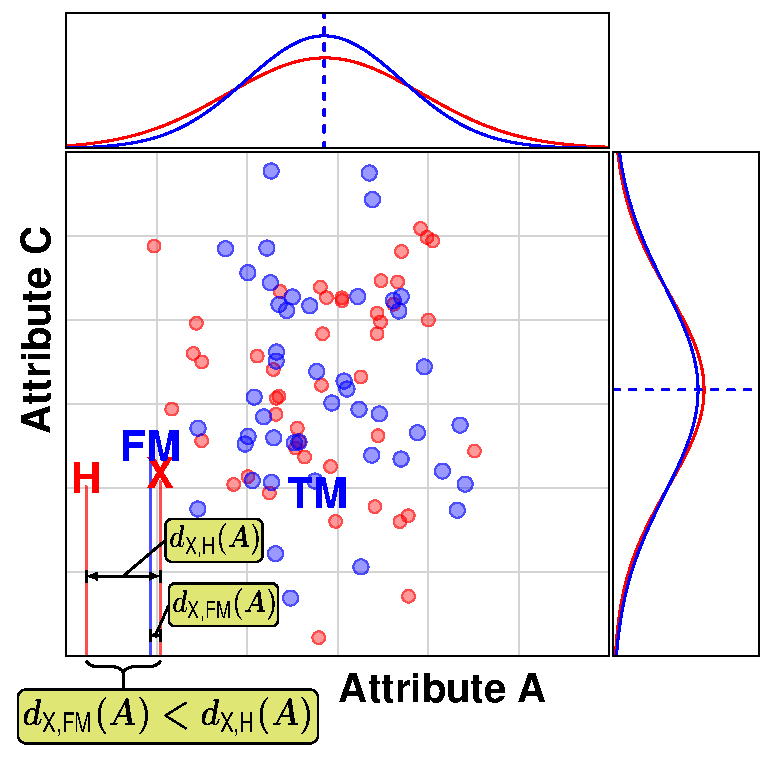
\includegraphics[width=0.8\textwidth]{glmSTIR_figure_2D_final_CvsA.pdf}}
%\end{minipage} \hspace{-0.4cm}
%\begin{minipage}[c]{0.5\textwidth}
%\centering
%\caption{{\bf Imposters vs true neighbors in the presence of interactions with three variables}. Scatter plot of simulated irrelevant Attribute C with a functional Attribute A {\bf(a)}. None of the attributes has a main effect, but Attribute B and C interact through differential correlation {\bf(b)}. Computing nearest neighbors with irrelevant attributes {\bf(a)} or lower dimensions leads to imposter nearest neighbors and degrades the ability of Relief-based methods to identify interaction effects. Computing distances in only these two dimensions leads to an imposter false miss (FM) for the nearest neighbor from the opposite outcome class for target instance X. This imposter leads to attribute A predicting closer projected distances for misses than hits (H), which incorrectly indicates that A is a poor discriminator (yellow boxes in {\bf a}). Computing nearest neighbors in higher dimensions {\bf(c-d)} or with the correct interaction partner leads to imposter nearest neighbor (FM) being replaced by the true nearest miss neighbor (TM) for target instance X, which correctly leads to attribute A predicting closer projected distances for hits (H) than misses, which is an indication that attribute A is a good discriminator (yellow boxes {\bf(b)}).}\label{fig:2dAvC}
%\end{minipage}
%%\end{center}
%\end{figure}

\newpage

\begin{figure}[ht!]
\begin{wrapfigure}{l}{0.6\textwidth}
    \vspace{-12pt}
	\centering
	\framebox{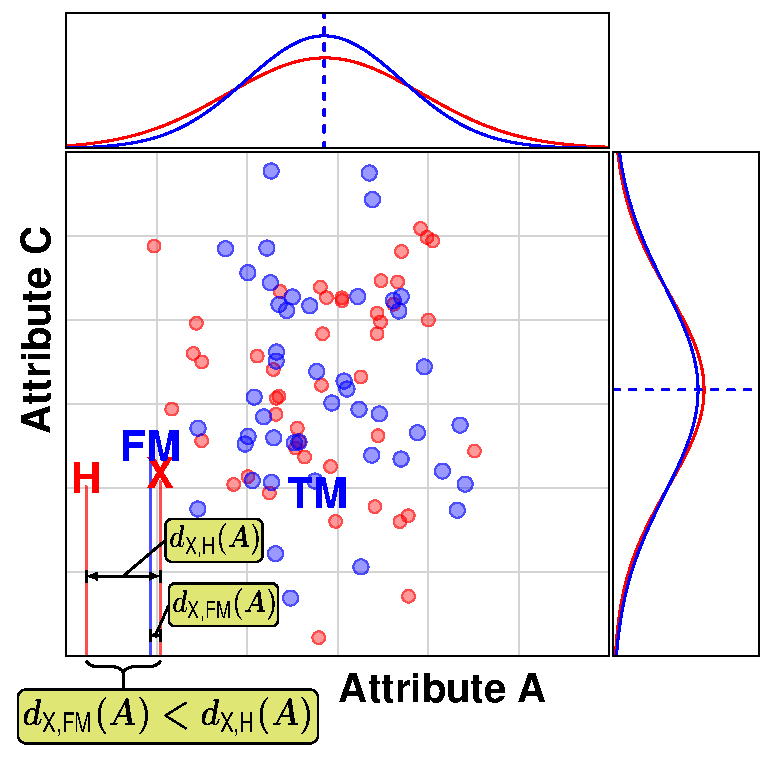
\includegraphics[width=0.55\textwidth]{glmSTIR_figure_2D_final_CvsA.pdf}}
\end{wrapfigure}
\noindent\refstepcounter{figure}\textbf{Fig \thefigure \label{fig:2dAvC}.} \textbf{Imposters vs true neighbors in the presence of interactions with three variables}. Scatter plot of simulated irrelevant Attribute C with a functional Attribute A \textbf{(a)}. None of the attributes has a main effect, but Attribute B and C interact through differential correlation \textbf{(b)}. Computing nearest neighbors with irrelevant attributes \textbf{(a)} or lower dimensions leads to imposter nearest neighbors and degrades the ability of Relief-based methods to identify interaction effects. Computing distances in only these two dimensions leads to an imposter false miss (FM) for the nearest neighbor from the opposite outcome class for target instance X. This imposter leads to attribute A predicting closer projected distances for misses than hits (H), which incorrectly indicates that A is a poor discriminator (yellow boxes in \textbf{(a)}). Computing nearest neighbors in higher dimensions \textbf{(c-d)} or with the correct interaction partner leads to imposter nearest neighbor (FM) being replaced by the true nearest miss neighbor (TM) for target instance X, which correctly leads to attribute A predicting closer projected distances for hits (H) than misses, which is an indication that attribute A is a good discriminator (yellow boxes \textbf{(b)}).
\end{figure}

Relief-based methods use information from all available attributes (omnigenic) to estimate an attribute's importance. However, if relevant higher-dimensional information is not used to establish the neighborhoods of instances, these methods will miss the effect of A because ``imposter'' neighbors will be used in the attribute estimate (False Miss (FM) in Fig.~\ref{fig:2dAvC}, where $d_{\text{X,FM}}(A)<d_{\text{X,H}}(A)$).  If one were to compute nearest neighbors in the A-C plane (ignoring the B dimension), the nearest miss would be an imposter (FM), which leads to a negative contribution to the importance score for A. One might call this C attribute a type-I confounding attribute because it increases the chances of interacting attributes to be false negatives. When nearest neighbors are calculated based on higher dimensions with relevant information (Fig.~\ref{fig:2dAvB}c), it is clear that TM is closer to X than FM. The imposter (FM) is replaced by the true nearest miss (TM) and attribute A correctly shows a greater projected difference between misses than hits (Fig.~\ref{fig:2dAvB}d $d_{\text{X,TM}}(A)>d_{\text{X,H}}(A)$), which is the signature of an important attribute. Univariate methods still cannot find the importance of A unless the interaction is explicitly modeled, but as long as functional variables A and B are in the space for nearest neighbor calculations (Fig.~\ref{fig:2dAvB}c-d), imposters can be excluded and Relief-based methods will find that A (and B) are important discriminators. 


[Ideas: Relating the increasing $k$ and myopic view to other distance-related method such as MDS/t-SNE vs PCA - local vs global distance - capturing non-linear manifold structure. \url{https://www.kdnuggets.com/2018/08/introduction-t-sne-python.html}]


\begin{figure}[ht!]
%%\begin{center}
\begin{minipage}[c]{0.4\textheight}
\centering 
		\framebox{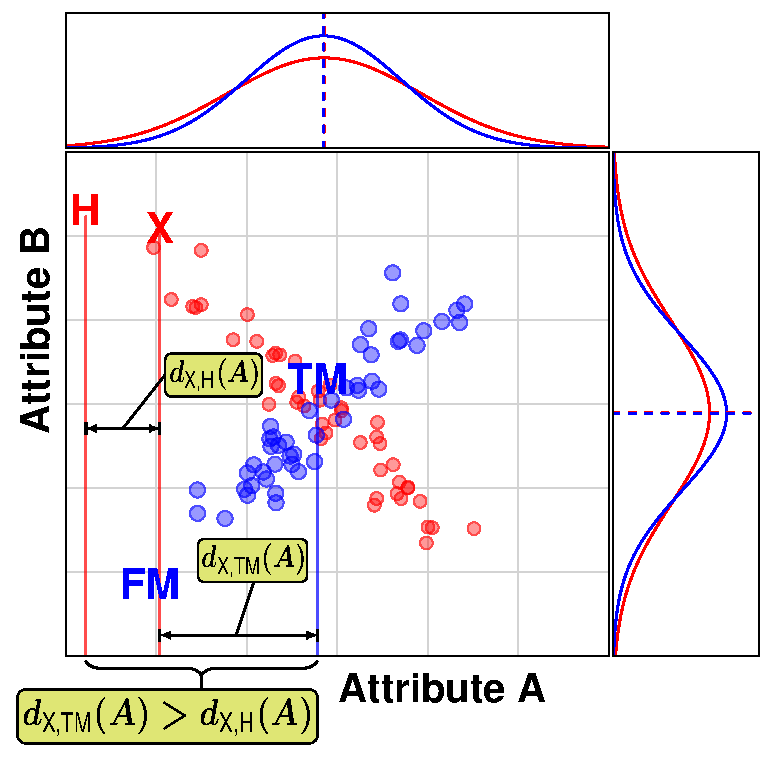
\includegraphics[width=0.8\textwidth]{glmSTIR_figure_2D_final_BvsA.pdf}}
\end{minipage} \hspace{-0.4cm}
\begin{minipage}[c]{0.5\textwidth}
\centering
\caption{{\bf True neighbors}}\label{fig:2dAvB}
\end{minipage}
%%\end{center}
\end{figure}  

\begin{figure}[ht!]
%%\begin{center}
\begin{minipage}[c]{0.4\textheight}
\centering
		\framebox{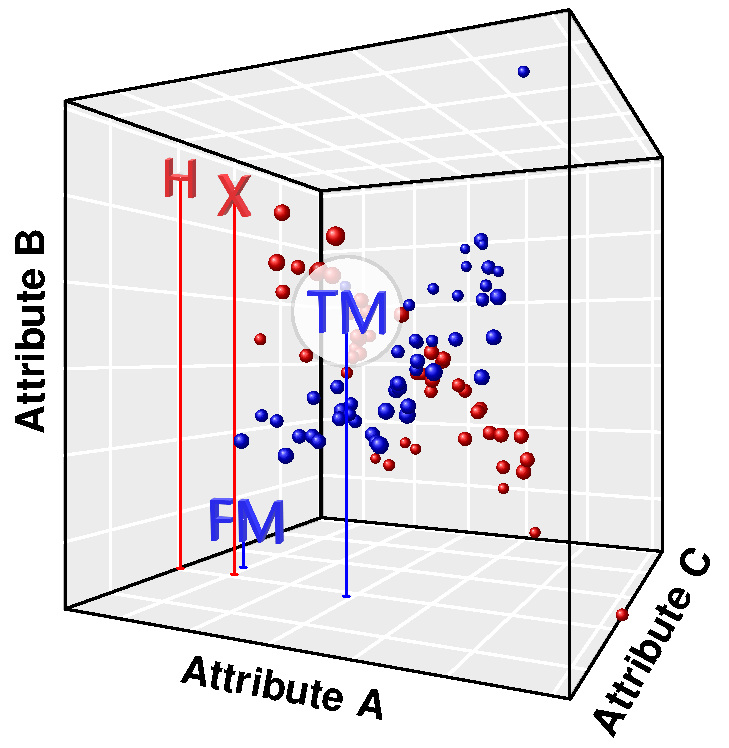
\includegraphics[width=0.8\textwidth]{nice_box_2D_points.pdf}}
\end{minipage} \hspace{-0.4cm}
\begin{minipage}[c]{0.5\textwidth}
\centering
\caption{{\bf 3D AB view}. Still working on this. }\label{fig:3d_c}
\end{minipage}
%%\end{center}
\end{figure}  

\begin{figure}[ht!]
%%\begin{center}
\begin{minipage}[c]{0.4\textheight}
\centering
		\framebox{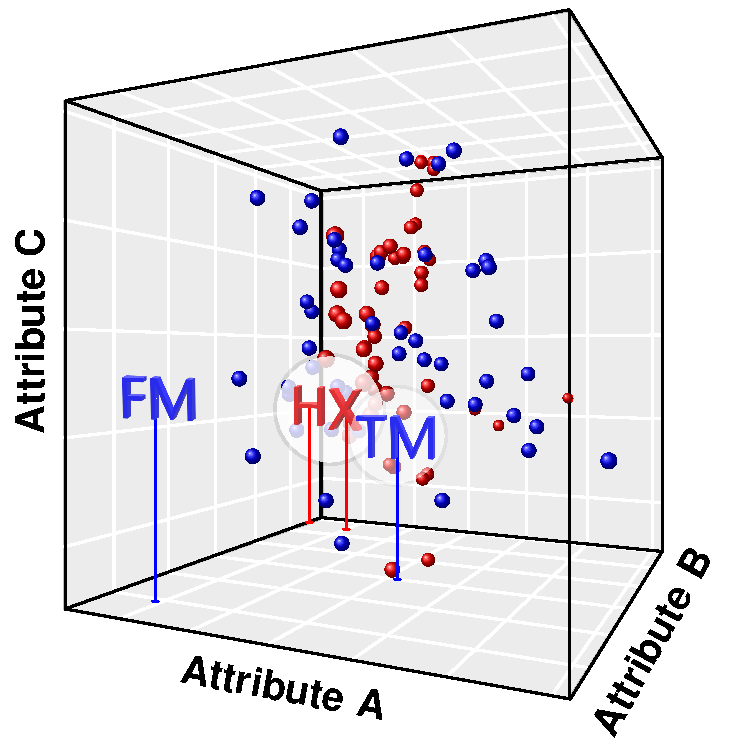
\includegraphics[width=0.8\textwidth]{nice_box_2D_points2.pdf}}
\end{minipage} \hspace{-0.4cm}
\begin{minipage}[c]{0.5\textwidth}
\centering
\caption{{\bf 3D AC view}. Still working on this. }\label{fig:3d_d}
\end{minipage}
%%\end{center}
\end{figure}  
Using same interaction, increase background noise genes to see degrading of A and B Relief importance because of curse of dimensionality (sparseness). 

\section{Neighborhood methods}
NPD methods rely on a neighborhood algorithm for feature selection. One may specify a fixed-$k$ number of neighbors, an average radius SURF, a multiSURF radius that adapts for each instance~\cite{urbanowicz17}, or a gene-wise adaptive-$k$. 

\section{Derivation of expected $k$ for multiSURF neighborhoods}
The multiSURF radius for an instance is the mean of its distances to all other instances subtracted by $\alpha=1/2$ of the standard deviation of this mean. Previously we showed empirically for balanced case-control datasets that a good constant-$k$ approximation to the expected number of neighbors within the multiSURF radii is $k=m/6$~\cite{stir}, where $m$ is the number of samples. Here we derive a more exact theoretical mean that shows the mathematical connection between neighbor-finding methods. This fixed-$k$ approximation to multi-SURF is independent of the type of data and the particular radii of each instance in the data.
%

The distance between instances $i$ and $j$ in the data set $X^{m \times p}$ of $m$ instances and $p$ attributes is calculated in the space of all attributes ($a \in \mathcal{A}$, $|\mathcal{A}|=p$) using a metric such as
\begin{equation}\label{eq:D}
% D^{(q)}_{ij}=\left(\sum_{a\in A}|\text{d}^{\text{type}}_{ij}(a)|^q\right)^{1/q},
D^{(q)}_{ij}=\left(\sum_{a\in \mathcal{A}}|\text{d}_{ij}(a)|^q\right)^{1/q},
\end{equation}
which is typically Manhattan ($q=1$) but may also be Euclidean ($q=2$). The quantity 
% $\text{d}^{\text{type}}_{ij}(a)$, 
$\text{d}_{ij}(a)$,
known as a ``$\text{diff}$'' in Relief literature, is the projection of the distance between instances $i$ and $j$ onto the attribute $a$ dimension. The 
% ``type'' refers to the data type of the attribute
function $\text{d}_{ij}(a)$ supports any type of attributes
(e.g., numeric and categorical).
For example, the projected difference between two instances $i$ and $j$ for a continuous numeric ($\text{d}^{\text{num}}$) attribute $a$ may be
%\begin{equation}\label{eq:diff}
%\text{diff}^{(\text{num})}(a,(\ri,\rj))=\frac{|\text{value}(a,\ri)-\text{value}(a,\rj)%|}{\max(a)-\min(a)}.
%\end{equation}
\begin{equation}\label{eq:diff}
\begin{aligned}
\text{d}^{\text{num}}_{ij}(a)&=\text{diff}(a,(i,j))\\
                                            & = {|\hat{X}_{ia}-\hat{X}_{ja}|},
\end{aligned}
\end{equation}
where $\hat{X}$ represents the standardized data matrix $X$.
We use a simplified d$_{ij}(a)$ notation in place of the $\text{diff}(a,(i,j))$ notation that is customary in Relief-based methods.
We omit the division by $\max(a)-\min(a)$ used by Relief to constrain scores to the interval from $-1$ to $1$.
As we show in subsequent sections, NPDR scores are standardized regression coefficients with corresponding P values, so any scaling operation at this stage is unnecessary for comparing attribute scores. 
%\emph{Omit: The scaling may alleviate bias in the distance calculation. However, standardizing the data matrix $X$ ($\hat{X}$) should have the same effect without division by $\max(a)-\min(a)$, which has usual distribution properties for distances (expand).}
The numeric d$^{\text{num}}_{ij}(a)$ projection is simply the absolute difference between row elements $i$ and $j$ of the data matrix $X^{m \times p}$ for the attribute column $a$. 

We define the NPDR neighborhood set $\mathcal{N}$ of ordered pair indices as follows. Instance $i$ is a point in $p$ dimensions, and we designate the topological neighborhood of $i$ as $N_{i}$. This neighborhood is a set of other instances trained on the data $X^{m \times p}$ and depends on the type of Relief neighborhood method (e.g., fixed-$k$ or adaptive radius) and the type of metric (e.g., Manhattan or Euclidean). If instance $j$ is in the neighborhood of $i$ ($j \in N_{i}$), then the ordered pair $(i,j) \in \mathcal{N}$ for the projected-distance regression analysis. The ordered pairs constituting the neighborhood can then be represented as nested sets:
\begin{equation}\label{eq:N}
\mathcal{N}=\{\{(i, j)\}_{i=1}^{m}\}_{\{j \ne i : j \in N_{i}\}}.
\end{equation}
The cardinality of the set $\{j \ne i : j \in N_{i}\}$ is $k_i$, the number of nearest neighbors for subject $i$. 

\subsection{Distribution of pairwise distances}
%Discuss Central Limit Theorem argument for the distribution being Gaussian. We can always say this is an assumption, but I think we can invoke the CLT. [I would be cautious here - TTL. We will be cautious invoking the CLT - BAM.]

Suppose that $X_{ia}, X_{ja} \overset{iid}{\sim} \mathcal{F}_X(\mu_X,\sigma^2_X)$ for two fixed and distinct instances $(i,j) \in \mathcal{N}$ and a fixed attribute $a \in \mathcal{A}$. 

It is clear that $|X_{ia} - X_{ja}|^q = |d_{ij}(a)|^q$ is another random variable. Let $Z^q_a \sim \mathcal{F}_{Z^q}(\mu_{z^q},\sigma^2_{z^q})$ be the random variable such that

\begin{equation}\label{eq:diffDistr}
Z^q_a = |d_{ij}(a)|^q = |X_{ia} - X_{ja}|^q, \quad a \in \mathcal{A}.
\end{equation}

Furthermore, the collection $\{Z^q_a | a \in \mathcal{A}\}$ is a random sample of size $p$ of mutually independent random variables. Hence, the sum of $Z^q_a$ over all $a \in \mathcal{A}$ is asymptotically normal by the Classical Central Limit Theorem (CCLT). More explicitly, this implies that

\begin{equation}\label{eq:DqAsympt}
\left(D^{(q)}_{ij}\right)^q = \sum_{a \in \mathcal{A}} |d_{ij}(a)|^q = \sum_{a \in \mathcal{A}} |X_{ia} - X_{ja}|^q = \sum_{a \in \mathcal{A}} Z^q_a \overset{.}{\sim} \mathcal{N}\left(\mu_{z^q}p,\sigma^2_{z^q}p\right)
\end{equation}

Consider the smooth function $g(z) = z^{1/q}$ that is continuously differentiable for $z>0$. Assuming that $\mu_{z^q}>0$, the Delta Method \cite{allStats} can be applied to show that 

\begin{equation}\label{eq:DqDeltaMethod}
\begin{aligned}
g\left(\left(D^{(q)}_{ij}\right)^q\right) &= g\left(\displaystyle \sum_{a \in \mathcal{A}}^{p}Z^q_a\right) \\
&= \left(\sum_{a \in \mathcal{A}} |X_{ia} - X_{ja}|^q\right)^{1/q} \\
&= D^{(q)}_{ij} \overset{.}{\sim} \mathcal{N}\left(g\left(\mu_{z^q}p\right),\left[g\prime \left(\mu_{z^q}p\right)\right]^2\sigma^2_{z^q}p\right) \\
\Rightarrow &\hphantom{=} D^{(q)}_{ij} \overset{.}{\sim} \mathcal{N}\left(\left(\mu_{z^q}p\right)^{1/q},\frac{\sigma^2_{z^q}p}{q^2\left(\mu_{z^q}p\right)^{2\left(1 - \frac{1}{q}\right)}}\right)
\end{aligned}
\end{equation}

For $q = 2$, a more accurate approximation of the sample mean is given by

\begin{equation}\label{eq:DqMeanImproved}
\text{E}\left(D^{(q)}_{ij}\right) = \left(\mu_{z^q}p - \frac{\sigma^2_{z^q}p}{q^2\left(\mu_{z^q}p\right)^{2\left(1 - \frac{1}{q}\right)}}\right)^{1/q}
\end{equation}

This is because

\begin{equation}\label{eq:DqImprovedExplaned}
\begin{aligned}
\text{E}\left(D^{(2)}_{ij}\right) &= \sqrt{\text{E}\left[\left(D^{(2)}_{ij}\right)^2\right] - \text{Var}\left(D^{(2)}_{ij}\right)} \\
&= \sqrt{\mu_{z^2}p - \frac{\sigma^2_{z^2}}{4\mu_{z^2}}}
\end{aligned}
\end{equation}

Therefore, the distance between two fixed and distinct instances $i$ and $j$ given by Eq. \ref{eq:D} is asymptotically normal.

One can readily verify the normality of distances between independent instances through sampling from any data distribution and plotting the histogram of pairwise distances. Histograms for the case of standard normal data and Manhattan ($q=1$) and Euclidean ($q=2$) metrics are shown in Figs. \ref{fig:manhattanConverge} and \ref{fig:euclideanConverge}, respectively. For these simulated distances, we fixed the number of instances $m=100$ and varied the number of attributes $p$ from 10 to 10000. For even a rather small number of predictors, as in the case of $p=10$, the sample distances are approximately normal. As $p$ increases, the normality becomes stronger.

\begin{figure}[ht!]
\centering
		\framebox{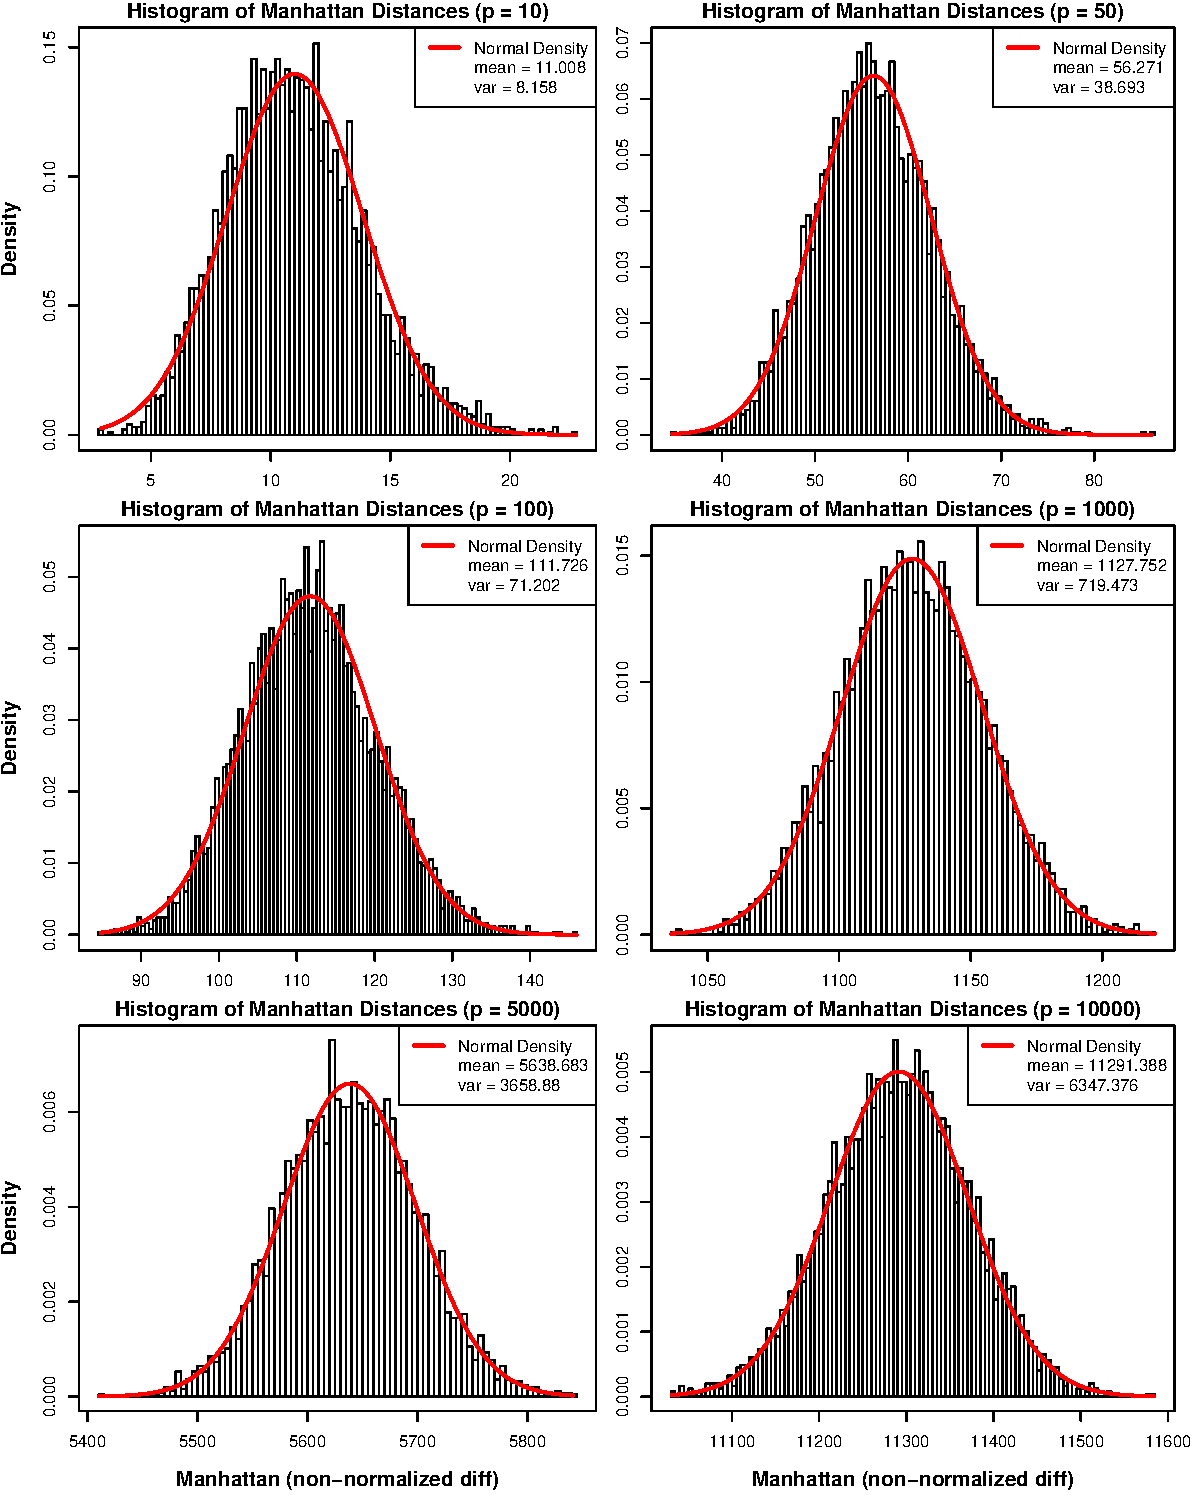
\includegraphics[width=0.95\textwidth]{central_limit_distances-Manhattan-Normal-diffstar.pdf}}
		\caption{Convergence to normality of Manhattan distances between iid random normal instances. For each simulated distance distribution, we fixed $m=100$ instances but varied $p$ from 10 to 10000. It is clear that convergence is rapid, and approximate normality can be safely assumed for even $p=10$.}\label{fig:manhattanConverge}
\end{figure} 

\begin{figure}[ht!]
\centering
		\framebox{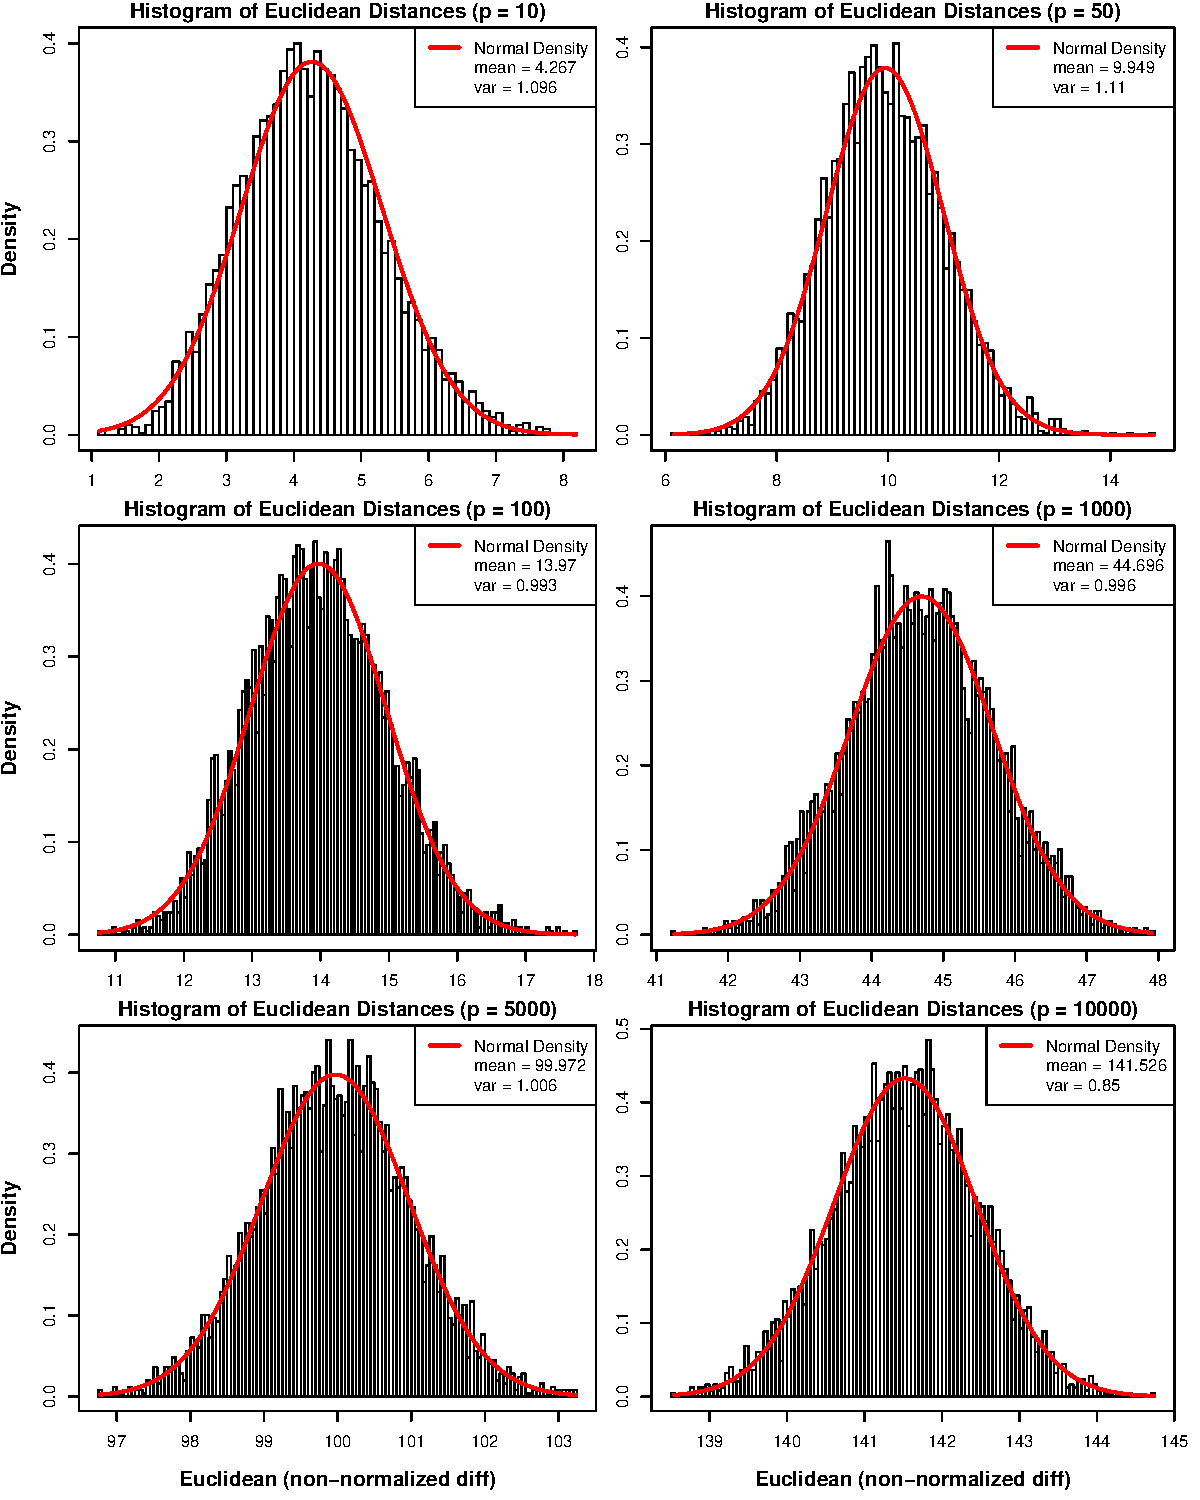
\includegraphics[width=0.95\textwidth]{central_limit_distances-Euclidean-Normal-diffstar.pdf}}
		\caption{Convergence to normality of Euclidean distances between iid random normal instances. For each simulated distance distribution, we fixed $m=100$ instances but varied $p$ from 10 to 10000. It is clear that convergence is rapid, and approximate normality can be safely assumed for even $p=10$.}\label{fig:euclideanConverge}
\end{figure}

For distance based learning methods, all pairwise distances are used to determine relative importances for attributes. The collection of all distances above the diagonal in an $m \times m$ distance matrix does not satisfy the independence assumption used in the previous derivations. This is because of the redundancy that is inherent to the distance matrix calcuation. However, this collection is still asymptotically normal with mean and variance approximately equal to those given in Eq. \ref{eq:DqDeltaMethod}. Hence, all fixed-radius methods will use a fixed radius that is some fraction of the expected pairwise distance for a given metric and data type. This implies that the probability of a fixed instance $j$ being within a fixed radius of a given instance $i$ can be parameterized by the expected pairwise distance and the variance of the pairwise distance. This probability is obtained by evaluating the normal cumulative distribution function (CDF), with corresponding mean and variance, at the quantile given by some function of the fixed radius. Therefore, we can derive the expected number of neighbors in the neighborhood of a fixed instance $i$. In other words, for sufficiently large data sets, the sample mean of the number of neighbors in a given neighborhood is well approximated by the product between the total number of possible neighbors and the expected probability of an instance being in a given neighborhood. The total number of possible neighbors for a fixed instance $i$ is always $m-1$, but this becomes approximately $\lfloor{\frac{m - 1}{2}}\rfloor$ when delineating between possible hits and misses for balanced data.

\subsection{Predicted number of neighbors in the multiSURF alpha neighborhood}

Regardless of the predictor data type (numeric or categorical), the distribution of the $p$ predictors (uniform, Gaussian, or binomial), or the metric used to compute distances (Manhattan or Euclidean), the $m(m-1)/2$ pairwise distances in the $p$-dimensional space are well approximated by a normal distribution. An instance $j$ is in the adaptive $\alpha$-radius neighborhood of $i$ ($j \in N^{\alpha}_{i}$) under the condition
%\begin{equation}
%\bar{D = \frac{2p}{\sqrt{\pi}}
%\end{equation}
%
%\begin{equation}
%\sigma_{D} = \frac{2p(\pi-2)}{\pi}
%\end{equation}
%
\begin{equation}
D_{ij} \le \, R_i^{\alpha} \implies j \in N^{\alpha}_{i},
\end{equation}
where the threshold radius for instance $i$ is
\begin{equation}
R_i^{\alpha} =  \bar{D}_i - \alpha \, \sigma_{\bar{D}_i}
\end{equation}
and
\begin{equation}
\bar{D}_i = \frac{1}{m-1} \sum_{j \ne i} D^{(\cdot)}_{ij}
\end{equation}
is the average of instance $i$'s pairwise distances (using Eq. D Equation) with standard deviation $\sigma_{\bar{D}_i}$. MultiSURF uses $\alpha=1/2$~\cite{msurf13}.

The probability of the remaining $m-1$ instances being inside the $\alpha$-radius of instance $i$ ($R_i^{\alpha}$) can be viewed as $m-1$ Bernoulli trials each with a probability of success $q_{\alpha}$. Then the average average number of neighbors is given by
\begin{equation}
\label{eq:binomial_average}
  {\bar{k}}_{\alpha} = (m-1)q_{\alpha},
\end{equation}
from the mean of a binomial random variable. To calculate $q_{\alpha}$, we assume the distribution of distances $(\{D_{ij} \}_{j \ne i})$ of neighbors of instance $i$ is normal $N(\bar{D}_i,\sigma_{\bar{D}_i})$. Our empirical studies confirm a normal distribution and that it is robust to data type and metric. Extreme violations of independence of attributes (extreme correlations or interactions) will cause the distribution to be right skewed, but this effect is difficult to observe in real data. Thus, for a Gaussian pairwise distance distribution, the probability $q_{\alpha}$ for one instance $j \ne i$ to be in the neighborhood of $i$ ($j \in N^{\alpha}_{i}$) is given by the area under the mean-centered ($\bar{D}_i$) Gaussian from $-\infty$ to $R_i^{\alpha}$. {\bf show Gaussian plot illustration?} An illustration of the area computed to estimate $q_{\alpha}$ is given by Fig. \ref{fig:gaussPlot}. This integral can be written in terms of the error function (erf):
\begin{equation}
\label{eq:q_prob}
q_{\alpha} = \frac{1}{2} \left( 1 - \mathrm{erf}\left( \frac{\alpha}{\sqrt{2}} \right) \right).
\end{equation}
And finally using Eqs. (\ref{eq:binomial_average} and \ref{eq:q_prob}) we find
\begin{equation}\label{eq:kbar}
{\bar{k}}_{\alpha} = \left \lfloor \frac{m-1}{2}  \left( 1 - \mathrm{erf}\left( \frac{\alpha}{\sqrt{2}} \right) \right) \right \rfloor,
\end{equation}
where we apply the floor to ensure the number of neighbors is integer. For data with balanced hits and misses in standard fixed-$k$ Relief, one divides this formula by 2. For multiSURF ($\alpha=1/2$), this formula gives $\bar{k}_{1/2}^{\text{hit/miss}} = \frac{1}{2}\bar{k}_{1/2} = .154 (m-1)$, which is very close to our previous empirical estimate $m/6$. When we compare multiSURF neighborhood methods with fixed-$k$ neighborhoods, we use $\bar{k}_{1/2}$. Using this $\alpha=1/2$ value has been shown to give good performance for simulated data sets. However, the best value for $\alpha$ is likely data-specific and may be determined through nested cross-validation and other parameter tuning methods.

\begin{figure}[ht!]
\centering
\begin{minipage}[h]{0.7\textwidth}
		\framebox{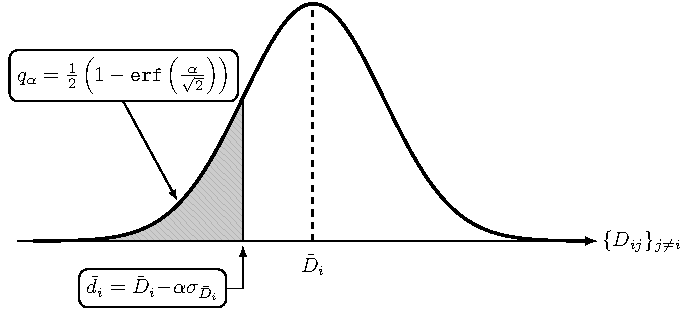
\includegraphics[width=0.95\textwidth]{shaded_bell_curve.pdf}}
\end{minipage}%\hspace{0.15cm}
\begin{minipage}[h]{0.3\textwidth}
\noindent\refstepcounter{figure}\textbf{Fig \thefigure \label{fig:gaussPlot}.} Illustration of the expected probability of a fixed instance $j$ being in the fixed radius neighborhood of another instance $i$. The fixed radius is parameterized by a fraction $\alpha$ of the standard deviation of all pairwise distances measured from instance $i$ to all possible neighbors.
\end{minipage}
\end{figure} 

\section{Derivation of means and standard deviations for metrics and data distributions}

\subsection{Distribution of \texorpdfstring{$|d_{ij}(a)|^q = |X_{ia} - X_{ja}|^q$}{}}

Suppose that $X_{ia}, X_{ja} \overset{iid}{\sim} \mathcal{F}_X(\mu_x,\sigma^2_x)$ and define $Z^q_a = |d_{ij}(a)|^q = |X_{ia} - X_{ja}|^q$, where $a \in \mathcal{A}$ and $|\mathcal{A}| = p$. In order to find the distribution of $Z^q_a$, we will use the following theorem given in \cite{freund2004}.

\begin{theorem}\label{thm:freund}
Let $f(x)$ be the value of the probability density of the continuous random variable $X$ at $x$. If the function given by $y = u(x)$ is differentiable and either increasing or decreasing for all values within the range of $X$ for which $f(x) \neq 0$, then, for these values of $x$, the equation $y = u(x)$ can be uniquely solved for $x$ to give $x = w(y)$, and for the corresponding values of $y$ the probability density of $Y = u(X)$ is given by

\[g(y) = f[w(y)] \cdot |w^\prime(y)| \quad \text{ provided } u^\prime(x) \neq 0\]

\noindent Elsewhere, $g(y) = 0$.
\end{theorem}

We have the following cases that result from solving for $X_{ja}$ in the equation given by $Z^q_a = |X_{ia} - X_{ja}|^q$.
\begin{itemize}
\item[(i)] Suppose that $X_{ja} = X_{ia} - \left(Z^q_a\right)^{1/q}$. Based on the iid assumption for $X_{ia}$ and $X_{ja}$, it follows from Thm. \ref{thm:freund} that the joint density function $g^{(1)}$ of $X_{ia}$ and $Z^q_a$ is given by

\begin{equation}
\begin{aligned}
g^{(1)}(x_{ia},z_a) &= f_X(x_{ia},x_{ja})\biggl|\frac{\partial x_{ja}}{\partial z_a}\biggr| \\
&= f_X(x_{ia})f_X(x_{ja})\biggl|\frac{-1}{q} \left(z^q_a\right)^{\frac{1}{q}-1}\biggr| \\
&= \frac{1}{q \left(z^q_a\right)^{1 - \frac{1}{q}}}f_X(x_{ia})f_X\left(x_{ia}-\left(z^q_a\right)^{1/q}\right), \quad z_a > 0
\end{aligned}
\end{equation}

The density function $f^{(1)}_{Z^q}$ of $Z^q_a$ is then defined as

\begin{equation}
\begin{aligned}
f^{(1)}_{Z^q}(z^q_a) &= \int_{-\infty}^{\infty} g^{(1)}(x_{ia},z^q_a)\text{d}x_{ia} \\
&= \frac{1}{q \left(z^q_a\right)^{1 - \frac{1}{q}}}\int_{-\infty}^{\infty} f_X(x_{ia})f_X\left(x_{ia}-\left(z^q_a\right)^{1/q}\right)\text{d}x_{ia}, \quad z_a > 0
\end{aligned}
\end{equation}

\item[(ii)] Suppose that $X_{ja} = X_{ia} + \left(Z^q_a\right)^{1/q}$. Based on the iid assumption for $X_{ia}$ and $X_{ja}$, it follows from Thm. \ref{thm:freund} that the joint density function $g^{(2)}$ of $X_{ia}$ and $Z_a$ is given by

\begin{equation}
\begin{aligned}
g^{(2)}(x_{ia},z_a) &= f_X(x_{ia},x_{ja})\biggl|\frac{\partial x_{ja}}{\partial z_a}\biggr| \\
&= f_X(x_{ia})f_X(x_{ja})\biggl|\frac{1}{q} \left(z^q_a\right)^{\frac{1}{q}-1}\biggr| \\
&= \frac{1}{q \left(z^q_a\right)^{1 - \frac{1}{q}}}f_X(x_{ia})f_X\left(x_{ia}-\left(z^q_a\right)^{1/q}\right), \quad z_a > 0
\end{aligned}
\end{equation}

The density function $f^{(2)}_{Z^q}$ of $Z^q_a$ is then defined as

\begin{equation}
\begin{aligned}
f^{(2)}_{Z^q}(z^q_a) &= \int_{-\infty}^{\infty} g^{(2)}(x_{ia},z^q_a)\text{d}x_{ia} \\
&= \frac{1}{q \left(z^q_a\right)^{1 - \frac{1}{q}}}\int_{-\infty}^{\infty} f_X(x_{ia})f_X\left(x_{ia}+\left(z^q_a\right)^{1/q}\right)\text{d}x_{ia}, \quad z_a > 0
\end{aligned}
\end{equation}
\end{itemize}

Let $F_{Z^q}$ denote the distribution function of the random variable $Z^q_a$. Furthermore, we define the events $E^{(1)}$ and $E^{(2)}$ as

\begin{equation}\label{eq:E(1)}
E^{(1)} = \bigl\{|X_{ia}-X_{ja}|^q \leq z^q_a | X_{ja} = X_{ia} - \left(Z^q_a\right)^{1/q}\bigr\}
\end{equation}

\noindent and

\begin{equation}\label{eq:E(2)}
E^{(2)} = \bigl\{|X_{ia}-X_{ja}|^q \leq z^q_a | X_{ja} = X_{ia} + \left(Z^q_a\right)^{1/q}\bigr\}.
\end{equation}

Then it follows from fundamental rules of probability that

\begin{equation}\label{eq:DqCDF}
\begin{aligned}
F_{Z^q}(z^q_a) &= \text{P}\left[Z^q_a \leq z^q_a\right] \\
&= \text{P}\left[|X_{ia} - X_{ja}|^q \leq z^q_a\right] \\
&= \text{P}\left[E^{(1)} \cup E^{(2)}\right] \\
&= \text{P}\bigl[E^{(1)}\bigr] + \text{P}\bigl[E^{(2)}\bigr] - \text{P}\bigl[E^{(1)} \cap E^{(2)}\bigr] \\
&= \text{P}\bigl[E^{(1)}\bigr] + \text{P}\bigl[E^{(2)}\bigr] \\
&= \int_{-\infty}^{z^q_a} f^{(1)}_{Z^q}(t) \text{d}t + \int_{-\infty}^{z^q_a} f^{(2)}_{Z^q}(t) \text{d}t \\
&= \int_{-\infty}^{z^q_a} \left(f^{(1)}_{Z^q}(t) + f^{(2)}_{Z^q}(t)\right) \text{d}t \\
&= \frac{1}{q \left(z^q_a\right)^{1 - \frac{1}{q}}}\int_{-\infty}^{z^q_a} \left(\int_{-\infty}^{\infty}f_X(x_{ia})\left[f_X(x_{ia} - t) + f_X(x_{ia} + t)\right] \text{d}x_{ia}\right)\text{d}t, \quad z_a > 0
\end{aligned}
\end{equation}

It follows directly from the result in Eq. \ref{eq:DqCDF} that the density function of the random variable $Z^q_a$ is given by

\begin{equation}\label{eq:DqPDF}
\begin{aligned}
f_{Z^q}(z^q_a) &= \frac{\partial}{\partial z^q_a} F_{Z^q}(z^q_a) \\
&= \frac{1}{q \left(z^q_a\right)^{1 - \frac{1}{q}}}\int_{-\infty}^{\infty} f_X(x_{ia})\left[f_X\left(x_{ia} - \left(z^q_a\right)^{1/q}\right) + f_X\left(x_{ia} + \left(z^q_a\right)^{1/q}\right)\right] \text{d}x_{ia}
\end{aligned}
\end{equation}
\noindent where $z_a > 0$.

Using Eq. \ref{eq:DqPDF}, we can compute the mean and variance of the random variable $Z^q_a$ as

\begin{equation}\label{eq:1DDqMean}
\mu_{z^q} = \int_{-\infty}^{\infty} z^q_a f_{Z^q}(z^q_a) \text{d}z^q_a
\end{equation}

\noindent and 

\begin{equation}\label{eq:1DDqVar}
\sigma^2_{z^q} = \int_{-\infty}^{\infty} \left(z^q_a\right)^2 f_{Z^q}(z^q_a) \text{d}z^q_a - \mu^2_{z^q}.
\end{equation}

It follows immediately from Eqs. \ref{eq:1DDqMean} and \ref{eq:1DDqVar} and the Classical Central Limit Theorem (CCLT) that

\begin{equation}\label{eq:DqDistr}
\left(D^{(q)}_{ij}\right)^q = \sum_{a \in \mathcal{A}} Z^q_a = \sum_{a \in \mathcal{A}} |X_{ia} - X_{ja}|^q \overset{.}{\sim} \mathcal{N}\left(\mu_{z^q}p,\sigma^2_{z^q}p\right)
\end{equation}

Applying the result given in Eq. \ref{eq:DqDeltaMethod}, the distribution of $D^{(q)}_{ij}$ is given by

\begin{equation}\label{eq:DDistr}
D^{(q)}_{ij} \overset{.}{\sim} \mathcal{N}\left(\left(\mu_{z^q}p\right)^{1/q},\frac{\sigma^2_{z^q}p}{q^2\left(\mu_{z^q}p\right)^{2\left(1 - \frac{1}{q}\right)}}\right), \quad \mu_{z^q} > 0
\end{equation}

\noindent with improved estimate of the mean for $q=2$ given by Eq. \ref{eq:DqMeanImproved}.

\subsubsection{Standard normal data}

If $X_{ia},X_{ja} \overset{iid}{\sim} \mathcal{N}(0,1)$, then the marginal density functions with respect to $X$ for $X_{ia}$, $X_{ia} - \left(Z^q_a\right)^{1/q}$, and $X_{ia} + \left(Z^q_a\right)^{1/q}$ are defined as

\begin{equation}\label{eq:normalXmarg}
f_X(x_{ia}) = \frac{1}{\sqrt{2\pi}}e^{-\frac{1}{2}x^2_{ia}},
\end{equation}

\begin{equation}\label{eq:normalXMinusZmarg}
f_X\left(x_{ia} - \left(z^q_a\right)^{1/q}\right) = \frac{1}{\sqrt{2\pi}}e^{-\frac{1}{2}\left(x_{ia} - \left(z^q_a\right)^{1/q}\right)^2}, \quad z_a > 0, \text{ and}
\end{equation}

\begin{equation}\label{eq:normalXPlusZmarg}
f_X\left(x_{ia} + \left(z^q_a\right)^{1/q}\right) = \frac{1}{\sqrt{2\pi}}e^{-\frac{1}{2}\left(x_{ia} + \left(z^q_a\right)^{1/q}\right)^2}, \quad z_a > 0
\end{equation}

Substituting the results given by Eqs. \ref{eq:normalXmarg}-\ref{eq:normalXPlusZmarg} into Eq. \ref{eq:DqPDF} and completing the square on $x_{ia}$ in the exponents, we have

%\begin{equation}\label{eq:normalPDF}
\begin{align}\label{eq:normalPDF}
  \begin{split}
  f_{Z^q}(z^q_a) &= \frac{1}{2 q \pi \left(z^q_a\right)^{1 - \frac{1}{q}}} e^{-\frac{1}{4}\left(z^q_a\right)^{2    /q}}\int_{-\infty}^{\infty} \biggl(e^{-\frac{1}{2}\left[\sqrt{2}x_{ia} - \frac{\sqrt{2}}{2}\left(z^q_a\right)^{1/q}\right]^2} \\
&\hspace{2in} + e^{-\frac{1}{2}\left[\sqrt{2}x_{ia} + \frac{\sqrt{2}}{2}\left(z^q_a\right)^{1/q}\right]^2}\biggr) \text{d}x_{ia}
\end{split} 
\\
&= \frac{1}{2 q \sqrt{\pi} \left(z^q_a\right)^{1 - \frac{1}{q}}} e^{-\frac{1}{4}\left(z^q_a\right)^{2/q}} \int_{-\infty}^{\infty}\frac{1}{\sqrt{2\pi}} \left(e^{-\frac{1}{2}u^2} + e^{-\frac{1}{2}u^2}\right) \text{d}u \\
&= \frac{1}{2 q \sqrt{\pi} \left(z^q_a\right)^{1 - \frac{1}{q}}} e^{-\frac{1}{4}\left(z^q_a\right)^{2/q}} (1 + 1) \\
&= \frac{1}{q \sqrt{\pi}}\left(z^q_a\right)^{\frac{1}{q} - 1} e^{-\frac{1}{4}\left(z^q_a\right)^{2/q}} \\
&= \frac{\frac{2}{q}}{\left(2^q\right)^{1/q} \Gamma\left(\frac{\frac{1}{q}}{\frac{2}{q}}\right)}\left(z^q_a\right)^{\frac{1}{q} - 1} e^{-\left(\frac{z^q_a}{2^q}\right)^{2/q}}
\end{align}
%\end{equation}

The density function given by Eq. \ref{eq:normalPDF} is a Generalized Gamma density with parameters $b = \frac{2}{q}$, $c = 2^q$, and $d = \frac{1}{q}$. This distribution has mean and variance given by

\begin{equation}\label{eq:1DnormalDqMean}
\begin{aligned}
\mu_{z^q} &= \frac{c\Gamma\left(\frac{d+1}{b}\right)}{\Gamma\left(\frac{d}{b}\right)} \\
&= \frac{2^q \Gamma\left(\frac{q + 1}{2}\right)}{\sqrt{\pi}}
\end{aligned}
\end{equation}

\noindent and

\begin{equation}\label{eq:1DnormalDqVar}
\begin{aligned}
\sigma^2_{z^q} &= c^2\left[\frac{\Gamma\left(\frac{d+2}{b}\right)}{\Gamma\left(\frac{d}{b}\right)} - \left(\frac{\Gamma\left(\frac{d+1}{b}\right)}{\Gamma\left(\frac{d}{b}\right)}\right)^2\right] \\
&= 4^{q}\left[\frac{\Gamma\left(q + \frac{1}{2}\right)}{\sqrt{\pi}} - \frac{\Gamma^2\left(\frac{1}{2}q + \frac{1}{2}\right)}{\pi}\right]
\end{aligned}
\end{equation}

By linearity of the expected value and variance operators under the iid assumption, Eqs. \ref{eq:1DnormalDqMean} and \ref{eq:1DnormalDqVar} allow the $p\text{-dimensional}$ mean and variance of the $D^{(q)}_{ij}$ distribution to be computed directly as

\begin{equation}\label{eq:normalDqMean}
\mu_{\left(D^{(q)}_{ij}\right)^q} = \text{E}\left[\left(D^{(q)}_{ij}\right)^q\right] = \text{E}\left(\sum_{a \in \mathcal{A}} Z^q_a\right) = \sum_{a \in \mathcal{A}} \text{E}\left(Z^q_a\right) = \sum_{a \in \mathcal{A}} \frac{2^q \Gamma\left(\frac{q + 1}{2}\right)}{\sqrt{\pi}} = \frac{2^q\Gamma\left(\frac{q + 1}{2}\right)}{\sqrt{\pi}}p
\end{equation}

\noindent and

\begin{equation}\label{eq:normalVar}
\begin{split}
\sigma^2_{\left(D^{(q)}_{ij}\right)^q} = \text{Var}\left[\left(D^{(q)}_{ij}\right)^q\right] &= \text{Var}\left(\sum_{a \in \mathcal{A}} Z^q_a\right) \\
&= \sum_{a \in \mathcal{A}} \text{Var}\left(Z^q_a\right) \\
&= \sum_{a \in \mathcal{A}} 4^{q}\left[\frac{\Gamma\left(q + \frac{1}{2}\right)}{\sqrt{\pi}} - \frac{\Gamma^2\left(\frac{1}{2}q + \frac{1}{2}\right)}{\pi}\right] \\
&= 4^{q}\left[\frac{\Gamma\left(q + \frac{1}{2}\right)}{\sqrt{\pi}} - \frac{\Gamma^2\left(\frac{1}{2}q + \frac{1}{2}\right)}{\pi}\right]p
\end{split}
\end{equation}

Therefore, the asymptotic distribution of $D^{(q)}_{ij}$ for standard normal data is

\begin{equation}\label{eq:normalDistr}
\mathcal{N}\left(\left(2^q\frac{\Gamma\left(\frac{q + 1}{2}\right)}{\sqrt{\pi}}p\right)^{1/q},
\frac{4^q p}{q^2 \left(\frac{2^q \Gamma\left(\frac{1}{2}q + \frac{1}{2}\right)}{\sqrt{\pi}}p\right)^{2\left(1 - \frac{1}{q}\right)}}\left[\frac{\Gamma\left(q + \frac{1}{2}\right)}{\sqrt{\pi}} - \frac{\Gamma^2\left(\frac{1}{2}q + \frac{1}{2}\right)}{\pi}\right]\right)
\end{equation}

\subsubsection{Standard uniform data}

If $X_{ia},X_{ja} \overset{iid}{\sim} \mathcal{U}(0,1)$, then the marginal density functions with respect to $X$ for $X_{ia}$, $X_{ia} - \left(Z^q_a\right)^{1/q}$, and $X_{ia} + \left(Z^q_a\right)^{1/q}$ are defined as

\begin{equation}\label{eq:uniformXmarg}
f_X(x_{ia}) = 1, \quad 0 \leq x_{ia} \leq 1
\end{equation}

\begin{equation}\label{eq:uniformXMinusZmarg}
f_X\left(x_{ia} - \left(z^q_a\right)^{1/q}\right) = 1, \quad 0 \leq x_{ia} - \left(z^q_a\right)^{1/q} \leq 1, \text{ and}
\end{equation}

\begin{equation}\label{eq:uniformXPlusZmarg}
f_X\left(x_{ia} + \left(z^q_a\right)^{1/q}\right) = 1, \quad 0 \leq x_{ia} + \left(z^q_a\right)^{1/q} \leq 1.
\end{equation}

Substituting the results given by Eqs. \ref{eq:uniformXmarg}-\ref{eq:uniformXPlusZmarg} into Eq. \ref{eq:DqPDF}, we have

\begin{equation}\label{eq:uniformDqPDF}
\begin{aligned}
f_{Z^q}(z^q_a) &= \frac{1}{q\left(z^q_a\right)^{1 - \frac{1}{q}}}\int_{-\infty}^{\infty}f_X(x_{ia})\left[f_X\left(x_{ia} - \left(z^q_a\right)^{1/q}\right) + f_X\left(x_{ia} + \left(z^q_a\right)^{1/q}\right)\right]\text{d}x_{ia},\\
& \hspace{4in} 0 < z_a \leq 1\\
&= \frac{1}{q\left(z^q_a\right)^{1 - \frac{1}{q}}}\int_{0}^{1}[f_X(x_{ia} - \left(z^q_a\right) + f_X\left(x_{ia} + \left(z^q_a\right)^{1/q}\right)]\text{d}x_{ia}, \quad 0 < z_a \leq 1 \\
&= \frac{1}{q\left(z^q_a\right)^{1 - \frac{1}{q}}}\int_{\left(z^q_a\right)}^{1}1\text{d}x_{ia} + \int_{0}^{1 - \left(z^q_a\right)}1\text{d}x_{ia}, \quad 0 < z_a \leq 1 \\
&= \frac{1}{q\left(z^q_a\right)^{1 - \frac{1}{q}}}\left[\left(1 - \left(z^q_a\right)\right) + \left(1 - \left(z^q_a\right)\right)\right], \quad 0 < z_a \leq 1 \\
&= \frac{1}{q} \cdot 2 \left(z^q_a\right)^{\frac{1}{q} - 1}\left[1 - \left(z^q_a\right)^{1/q}\right]^{2 - 1}, \quad 0 < z_a \leq 1
\end{aligned}
\end{equation}

The density given by Eq. \ref{eq:uniformDqPDF} is a Kumaraswamy density with parameters $b = \frac{1}{q}$ and $c = 2$ with moment generating function (MGF) given by

\begin{equation}\label{eq:uniformDqMGF}
\begin{aligned}
M_n &=  \frac{c\Gamma\left(1 + \frac{n}{b}\right) \Gamma(c)}{\Gamma\left(1 + c + \frac{n}{b}\right)}\\
&= \frac{2}{(nq + 2)(nq + 1)}
\end{aligned}
\end{equation}

Using the MGF given by Eq. \ref{eq:uniformDqMGF}, the mean and variance of $Z^q_a$ are computed as

\begin{equation}\label{eq:1DuniformDqMean}
\mu_{z^q} = \frac{2}{(q + 2)(q + 1)}
\end{equation}

\noindent and

\begin{equation}\label{eq:1DuniformDqVar}
\sigma^2_{z^q} = \frac{1}{(q + 1)(2q + 1)} - \left(\frac{2}{(q + 2)(q + 1)}\right)^2
\end{equation}

By linearity of the expected value and variance operators under the iid assumption, Eqs. \ref{eq:uniformDqMean} and \ref{eq:uniformDqVar} allow the $p \text{-dimensional}$ mean and variance of the $\left(D^{(q)}_{ij}\right)^q$ distribution to be computed directly as

\begin{equation}\label{eq:uniformDqMean}
\begin{split}
\mu_{\left(D^{(q)}_{ij}\right)^q} = \text{E}\left[\left(D^{(q)}_{ij}\right)^q\right] &= \text{E}\left(\sum_{a \in \mathcal{A}}Z^q_a\right) \\
&= \sum_{a \in \mathcal{A}} \text{E}(Z^q_a) \\
&= \sum_{a \in \mathcal{A}} \frac{2}{(q + 2)(q + 1)} \\
&= \frac{2p}{(q + 2)(q + 1)}
\end{split}
\end{equation}

\noindent and

\begin{equation}\label{eq:uniformDqVar}
\begin{split}
\sigma^2_{\left(D^{(q)}_{ij}\right)^q} = \text{Var}\left[\left(D^{(q)}_{ij}\right)^q\right] &= \text{Var}\left(\sum_{a \in \mathcal{A}} Z^q_a\right) \\
&= \sum_{a \in \mathcal{A}} \text{Var}\left(Z^q_a\right) \\
&= \sum_{a \in \mathcal{A}} \left[\frac{1}{(q + 1)(2q + 1)} - \left(\frac{2}{(q + 2)(q + 1)}\right)^2\right] \\
&= \left[\frac{1}{(q + 1)(2q + 1)} - \left(\frac{2}{(q + 2)(q + 1)}\right)^2\right]p
\end{split}
\end{equation}

Therefore, the asymptotic distribution of $D^{(q)}_{ij}$ for standard uniform data is

\begin{equation}\label{eq:uniformDistr}
\begin{split}
\mathcal{N}{\text{\LARGE $\Biggl($}}& \left(\frac{2p}{(q + 2)(q + 1)}\right)^{1/q}, \\
& \frac{p}{q^2\left(\frac{2p}{(q + 2)(q + 1)}\right)^{2\left(1 - \frac{1}{q}\right)}}\left[\frac{1}{(q + 1)(2q + 1)} - \left(\frac{2}{(q + 2)(q + 1)}\right)^2\right]{\text{\LARGE $\Biggr)$}}.
\end{split}
\end{equation}

\subsection{Manhattan \texorpdfstring{($q=1$)}{}}

With our general formulas for the asymptotic mean and variance given by Eqs. \ref{eq:normalDistr} and \ref{eq:uniformDistr} for any value of $q \in \mathbb{Z}^+$, we can simply substitute a particular value of $q$ in order to determine the asymptotic distribution of the corresponding distance metric $D^{(q)}_{ij}$. We demonstrate this with the example of the Manhattan ($q=1$) metric for standard normal and standard uniform data.

\subsubsection{Standard normal data}

Using the mean given by Eq. \ref{eq:normalDistr} and substituting $q=1$, we have the following for standard normal data

\begin{equation}\label{eq:normalManMean}
\begin{aligned}
\text{E}\left(D^{(1)}_{ij}\right) &= \left(2\frac{\Gamma\left(\frac{1 + 1}{2}\right)}{\sqrt{\pi}}p\right)^{1/1} \\
&= \frac{2p}{\sqrt{\pi}}\Gamma(1) \\
&= \frac{2p}{\sqrt{\pi}}
\end{aligned}
\end{equation}

Similarly, the variance of $D^{(1)}_{ij}$ is given by

\begin{equation}\label{eq:normalManVar}
\begin{aligned}
\text{Var}\left(D^{(1)}_{ij}\right) &= \frac{4^1p}{1^2\left(\frac{2^1\Gamma\left(\frac{1}{2}(1) + \frac{1}{2}\right)}{\sqrt{\pi}}p\right)^{2\left(1 - \frac{1}{1}\right)}}\left[\frac{\Gamma\left(1 + \frac{1}{2}\right)}{\sqrt{\pi}} - \frac{\Gamma^2\left(\frac{1}{2}(1) + \frac{1}{2}\right)}{\pi}\right] \\
&= \frac{4p}{1}\left[\frac{\frac{1}{2}\Gamma\left(\frac{1}{2}\right)}{\sqrt{\pi}} - \frac{\Gamma^2(1)}{\pi}\right] \\
&= 4p\left[\frac{1}{2} - \frac{1}{\pi}\right] \\
&= \frac{2(\pi - 2)p}{\pi}
\end{aligned}
\end{equation}

\subsubsection{Standard uniform data}

Using the mean given by Eq. \ref{eq:uniformDistr} and substituting $q=1$, we have the following for standard uniform data

\begin{equation}\label{eq:uniformManMean}
\begin{aligned}
\text{E}\left(D^{(1)}_{ij}\right) &= \left(\frac{2p}{(1+2)(1+1)}\right)^{1/1} \\
&= \frac{2p}{6} \\
&= \frac{p}{3}
\end{aligned}
\end{equation}

Similarly, the variance of $D^{(1)}_{ij}$ is given by

\begin{equation}\label{eq:uniformManVar}
\begin{aligned}
\text{Var}\left(D^{(1)}_{ij}\right) &= \frac{p}{1^2\left(\frac{2p}{(1 + 2)(1 + 1)}\right)^{2\left(1 - \frac{1}{1}\right)}}\left[\frac{1}{(1 + 1)(2(1) + 1)} - \left(\frac{2}{(1 + 2)(1 + 1)}\right)^2\right] \\
&= p\left[\frac{1}{6} - \frac{1}{9}\right] \\
&= \frac{p}{18}
\end{aligned}
\end{equation}

\subsection{Euclidean \texorpdfstring{($q=2$)}{}}

Analogous to the previous section, we demonstrate the usage of Eqs. \ref{eq:normalDistr} and \ref{eq:uniformDistr} for the Euclidean ($q=2$) metric for standard normal and standard uniform data.

\subsubsection{Standard normal data}

Using the mean given by Eq. \ref{eq:normalDistr} and substituting $q=2$, we have the following for standard normal data

\begin{equation}\label{eq:normalEucMean}
\begin{aligned}
\text{E}\left(D^{(2)}_{ij}\right) &= \left(2\frac{\Gamma\left(\frac{2 + 1}{2}\right)}{\sqrt{\pi}}p\right)^{1/2} \\
&= \left(\frac{2p}{\sqrt{\pi}}\Gamma\left(\frac{3}{2}\right)\right)^{1/2} \\
&= \sqrt{2p}
\end{aligned}
\end{equation}

Similarly, the variance of $D^{(2)}_{ij}$ is given by

\begin{equation}\label{eq:normalEucVar}
\begin{aligned}
\text{Var}\left(D^{(1)}_{ij}\right) &= \frac{4^2p}{2^2\left(\frac{2^2\Gamma\left(\frac{1}{2}(2) + \frac{1}{2}\right)}{\sqrt{\pi}}p\right)^{2\left(1 - \frac{1}{2}\right)}}\left[\frac{\Gamma\left(2 + \frac{1}{2}\right)}{\sqrt{\pi}} - \frac{\Gamma^2\left(\frac{1}{2}(2) + \frac{1}{2}\right)}{\pi}\right] \\
&= \frac{16p}{4\left(\frac{4\Gamma\left(\frac{3}{2}\right)}{\sqrt{\pi}}p\right)}\left[\frac{\Gamma\left(\frac{5}{2}\right)}{\sqrt{\pi}} - \frac{\Gamma^2\left(\frac{3}{2}\right)}{\pi}\right] \\
&= 2\left[\frac{3}{4} - \frac{1}{4}\right] \\
&= 1 
\end{aligned}
\end{equation}

For the case in which the number of attributes $p$ is small, an improved estimate of the mean is given by Eq. \ref{eq:DqMeanImproved}. The lower dimensional estimate of the mean is as follows.

\begin{equation}\label{eq:normalEucMeanImproved}
\begin{aligned}
\text{E}\left(D^{(2)}_{ij}\right) &= \left(2\frac{\Gamma\left(\frac{2 + 1}{2}\right)}{\sqrt{\pi}}p - 1\right)^{1/2} \\
&= \left(\frac{2p}{\sqrt{\pi}}\Gamma\left(\frac{3}{2}\right) - 1\right)^{1/2} \\
&= \sqrt{2p - 1}
\end{aligned}
\end{equation}

For high dimensional data sets, such as gene expression, rs-fMRI, or GWAS, it is clear that the magntiude of $p$ will be sufficient to use Eq. \ref{eq:normalEucMean} since $\sqrt{2p} \approx \sqrt{2p - 1}$ in that case.

\subsubsection{Standard uniform data}

Using the mean given by Eq. \ref{eq:uniformDistr} and substituting $q=2$, we have the following for standard uniform data

\begin{equation}\label{eq:uniformEucMean}
\begin{aligned}
\text{E}\left(D^{(2)}_{ij}\right) &= \left(\frac{2p}{(2+2)(2+1)}\right)^{1/2} \\
&= \left(\frac{2p}{12}\right)^{1/2} \\
&= \sqrt{\frac{p}{6}}
\end{aligned}
\end{equation}

Similarly, the variance of $D^{(2)}_{ij}$ is given by

\begin{equation}\label{eq:uniformEucVar}
\begin{aligned}
\text{Var}\left(D^{(2)}_{ij}\right) &= \frac{p}{2^2\left(\frac{2p}{(2 + 2)(2 + 1)}\right)^{2\left(1 - \frac{1}{2}\right)}}\left[\frac{1}{(2 + 1)(2(2) + 1)} - \left(\frac{2}{(2 + 2)(2 + 1)}\right)^2\right] \\
&= \frac{3p}{2}\left[\frac{1}{15} - \frac{1}{36}\right] \\
&= \frac{7p}{120}
\end{aligned}
\end{equation}

For the case in which the number of attributes $p$ is small, an improved estimate of the mean is given by Eq. \ref{eq:DqMeanImproved}. The lower dimensional estimate of the mean is as follows.

\begin{equation}\label{eq:uniformEucMeanImproved}
\begin{aligned}
\text{E}\left(D^{(2)}_{ij}\right) &= \left(\frac{2p}{(2+2)(2+1)} - \frac{7}{120}\right)^{1/2} \\
&= \left(\frac{2p}{12} - \frac{7}{120}\right)^{1/2} \\
&= \sqrt{\frac{p}{6} - \frac{7}{120}}
\end{aligned}
\end{equation}

For high dimensional data sets, such as gene expression, rs-fMRI, or GWAS, it is clear that the magntiude of $p$ will be sufficient to use Eq. \ref{eq:normalEucMean} since $\sqrt{\frac{p}{6}} \approx \sqrt{\frac{p}{6} - \frac{7}{120}}$ in that case.

\subsection{Distribution of attribute extremes}

For Relief-based methods \cite{robnik2003,urbanowiczReliefReview2018}, the standard numeric diff metric is given by

\begin{equation}\label{eq:normDiff}
d^{\text{num}}_{ij}(a) = \text{diff}(a,(i,j)) = \frac{|X_{ia} - X_{ja}|}{\text{max}(a) - \text{min}(a)}
\end{equation}

\noindent where $\text{max}(a) = \displaystyle \max_{k \in \mathcal{I}}\{X_{ka}\}$, $\text{min}(a) = \displaystyle \min_{k \in \mathcal{I}}\{X_{ka}\}$, and $\mathcal{I} = \{1,2,\dots,m\}$. 

In order to determine moments of asymptotic distance distributions induced by Eq. \ref{eq:normDiff}, we must first derive the asymptotic extreme value distributions of the attribute maximum and minimum. Although the exact distribution of the maximum or minimum requires an assumption about the data distribution, the Fisher-Tippett-Gnedenko Theorem allows us to categorize the extreme value distribution for a collection of independent and identically distributed random variables into one of three distributional families. Before stating the theorem, we first need the following definition.

\begin{definition}
A distribution $\mathcal{F}_X$ is said to be \textbf{degenerate} if its density function $f_X$ is the Dirac delta $\delta(x - c_0)$ centered at a constant $c_0 \in \mathbb{R}$, with corresponding distribution function $F_X$ defined as

\[F_X(x)\begin{cases}
          1, & x \geq c_0, \\
          0, & x < c_0.
        \end{cases}
\]
\end{definition}

\begin{theorem}[Fisher-Tippett-Gnedenko]\label{thm:EVT}
Let $X_{1a},X_{2a},\dots,X_{ma} \overset{iid}{\sim} \mathcal{F}_X\left(\mu_x,\sigma^2_x\right)$ and let $X^\alpha_a = \displaystyle \max_{k \in \mathcal{I}}\{X_{ka}\}$. If there exists two non-random sequences $b_m>0$ and $c_m$ such that

\[\lim_{m \to \infty} \text{P}\left(\frac{X^\alpha_a - c_m}{b_m} \leq x\right) = G_X(x),\]

\noindent where $G_X$ is a non-degenerate distribution function, then the limiting distribution $\mathcal{G}_X$ is in the Gumbel, Fr\'{e}chet, or Wiebull family.
\end{theorem}

The three distribution families given in Thm. \ref{thm:EVT} are actually special cases of the Generalized Extreme Value Distribution. In the context of extreme values, Thm. \ref{thm:EVT} is analogous to the Central Limit Theorem for the distribution of sample mean. We will take advantage of this theorem for the distribution of the maximum for standard normal data to show that the limiting distribution is in the Gumbel family. However, we will derive the distribution of the maximum and minimum for standard uniform data directly. Regardless of data type, the distribution of the sample maximum is derived in Eq. \ref{eq:exact_max}.

\begin{equation}\label{eq:exact_max}
\begin{aligned}
\text{P}[X^\alpha_a \leq x] &= \text{P}\left[\max_{k \in \mathcal{I}}\{X_{ka}\} \leq x\right] \\
&= \text{P}[X_{1a} \leq x, X_{2a} \leq x, \dots, X_{ma} \leq x] \\
&= \prod_{k = 1}^{m} \text{P}[X_{ka} \leq x] \\
&= \prod_{k=1} F_X(x) \\
&= [F_X(x)]^m
\end{aligned}
\end{equation}

Therefore, we have the following expression for the distribution function of the maximum.

\begin{equation}\label{eq:exact_max_distr_fn}
F_\text{max}(x) = [F_X(x)]^m
\end{equation}

Differentiating the distribution function given by Eq. \ref{eq:exact_max_distr_fn} gives us the following density function for the distribution of the maximum.

\begin{equation}\label{eq:exact_max_dens_fn}
\begin{aligned}
f_\text{max}(x) &= \frac{\text{d}}{\text{d}x} F_\text{max}(x) \\
&= \frac{\text{d}}{\text{d}x} [F_X(x)]^m \\
&= m [F_X(x)]^{m-1} f_X(x)
\end{aligned}
\end{equation}

The distribution of the sample minimum, $X^\omega_a$, is derived in Eq. \ref{eq:exact_min}.

\begin{equation}\label{eq:exact_min}
\begin{aligned}
\text{P}[X^\omega_a \leq x] &= 1 - \text{P}[X^\omega_a \geq x] \\
&= 1 - \text{P}\left[\min_{k \in \mathcal{I}}\{X_{ka}\} \geq x\right] \\
&= 1 - \text{P}[X_{1a} \geq x, X_{2a} \geq x, \dots, X_{ma} \geq x] \\
&= 1 - \prod_{k=1}^{m}\text{P}[X_{ka} \geq x] \\
&= 1 - \left[\text{P}[X_{1a} \geq x]\right]^m \\
&= 1 - \left[1 - \text{P}[X_{1a} \leq x]\right]^m \\
&= 1 - \left[1 - F_X(x)\right]^m
\end{aligned}
\end{equation}

Therefore, we have the following expression for the distribution function of the minimum.

\begin{equation}\label{eq:exact_min_distr_fn}
F_\text{min}(x) = 1 - [1 - F_X(x)]^m
\end{equation}

Differentiating the distribution function given by Eq. \ref{eq:exact_min_distr_fn} gives us the following density function for the distribution of the minimum.

\begin{equation}\label{eq:exact_min_dens_fn}
\begin{aligned}
f_\text{min}(x) &= \frac{\text{d}}{\text{d}x} F_\text{min}(x) \\
&= \frac{\text{d}}{\text{d}x} \left(1 - [1 - F_X(x)]^m\right) \\
&= m\left[1 - F_X(x)\right]^{m-1}f_X(x)
\end{aligned}
\end{equation}

Given the densities of the distribution of sample maximum and minimum, we can easily compute moments and the variance. The first and second moment about the origin and the variance of the distribution of the maximum are given by the following.

\begin{equation}\label{eq:mu_max}
\begin{aligned}
\mu^{(1)}_\alpha(m) = \text{E}(X^\alpha_a) &= \int_{-\infty}^{\infty}x f_\text{max}(x)\text{d}x \\
&= \int_{-\infty}^{\infty}x \left(m [F_X(x)]^{m-1} f_X(x)\right)\text{d}x \\
&= m \int_{-\infty}^{\infty}x f_X(x) [F_X(x)]^{m-1}\text{d}x
\end{aligned}
\end{equation}

\begin{equation}\label{eq:mu2_max}
\begin{aligned}
\mu^{(2)}_\alpha(m) = \text{E}[(X^\alpha_a)^2] &= \int_{-\infty}^{\infty}x^2 f_\text{max}(x)\text{d}x \\
&= \int_{-\infty}^{\infty}x^2 \left(m [F_X(x)]^{m-1} f_X(x)\right)\text{d}x \\
&= m \int_{-\infty}^{\infty}x^2 f_X(x) [F_X(x)]^{m-1}\text{d}x
\end{aligned}
\end{equation}

\begin{equation}\label{eq:sig_max}
\sigma^2_\alpha(m) = \mu^{(2)}_\alpha(m) - \left[\mu^{(1)}_\alpha(m)\right]^2
\end{equation}

Similarly, we have the first and second moment about the origin and variance of the distribution of sample minimum given by the following.

\begin{equation}\label{eq:mu_min}
\begin{aligned}
\mu^{(1)}_\omega(m) = \text{E}(X^\omega_a) &= \int_{-\infty}^{\infty}x f_\text{min}(x)\text{d}x \\
&= \int_{-\infty}^{\infty}x \left(m [F_X(x)]^{m-1} f_X(x)\right)\text{d}x \\
&= m \int_{-\infty}^{\infty}x f_X(x) [F_X(x)]^{m-1}\text{d}x
\end{aligned}
\end{equation}

\begin{equation}\label{eq:mu2_min}
\begin{aligned}
\mu^{(2)}_\omega(m) = \text{E}[(X^\omega_a)^2] &= \int_{-\infty}^{\infty}x^2 f_\text{min}(x)\text{d}x \\
&= \int_{-\infty}^{\infty}x^2 \left(m [F_X(x)]^{m-1} f_X(x)\right)\text{d}x \\
&= m \int_{-\infty}^{\infty}x^2 f_X(x) [F_X(x)]^{m-1}\text{d}x
\end{aligned}
\end{equation}

\begin{equation}\label{eq:sig_min}
\sigma^2_\omega(m) = \mu^{(2)}_\omega(m) - \left[\mu^{(1)}_\omega(m)\right]^2
\end{equation}

With the densities of attribute maximum and minimum for sample size $m$, the expected range is given by the following.

\begin{equation}\label{eq:exp_rng}
\begin{aligned}
\text{E}(X^\alpha_a - X^\omega_a) &= \text{E}(X^\alpha_a) - \text{E}(X^\omega_a) \\
&= \mu^{(1)}_\alpha(m) - \mu^{(1)}_\omega(m)
\end{aligned}
\end{equation}

For a data distribution that has zero skewness and has support that is symmetric about 0, the result given by Eq. \ref{eq:exp_rng} can be simplified to the following expression.

\begin{equation}\label{eq:exp_rng_symm}
\text{E}(X^\alpha_a - X^\omega_a) = 2 \mu^{(1)}_\alpha(m)
\end{equation}

For large samples ($m >> 1$), the covariance between the sample maximum and minimum is approximately zero \cite{gumbel1947}. Therefore, the variance of the attribute range of a sample of size $m$ is given by the following.

\begin{equation}\label{eq:var_rng}
\begin{aligned}
\text{Var}(X^\alpha_a - X^\omega_a) &\approx \text{Var}(X^\alpha_a) + \text{Var}(X^\omega_a) \\
&= \sigma^2_\alpha(m) + \sigma^2_\omega(m)
\end{aligned}
\end{equation}

Under the assumption of zero skewness and support that is symmetric about 0, the result given by Eq. \ref{eq:var_rng} becomes the following.

\begin{equation}\label{eq:var_rng_symm}
\begin{aligned}
\text{Var}(X^\alpha_a - X^\omega_a) &= 2 \text{Var}(X^\alpha_a) \\
&= 2 \sigma^2_\alpha
\end{aligned}
\end{equation}

Let $\mu_{D^{(q)}_{ij}}$ and $\sigma^2_{D^{(q)}_{ij}}$ denote the mean and variance given by Eq. \ref{eq:DDistr}. Furthermore, let $D^{(q*)}_{ij}$ denote the max-min normalized distance between instances $i$ and $j$ that is induced by the metric given by Eq. \ref{eq:normDiff}. Then the mean of the max-min normalized distance distribution is given by the following.

\begin{equation}\label{eq:max-min_D_mean}
\begin{aligned}
\mu_{D^{(q*)}_{ij}} &= \text{E}\left[\left(\sum_{a \in \mathcal{A}}\left(\frac{|X_{ia} - X_{ja}|}{X^\alpha_a - X^\omega_a}\right)^q\right)^{1/q}\right] \\
&\approx \frac{1}{\text{E}(X^\alpha_a - X^\omega_a)}\text{E}\left[\left(\sum_{a \in \mathcal{A}}|X_{ia} - X_{ja}|^q\right)^{1/q}\right] \\
&= \frac{\mu_{D^{(q)}_{ij}}}{\text{E}(X^\alpha_a) - \text{E}(X^\omega_a)} \\
&= \frac{\mu_{D^{(q)}_{ij}}}{\mu^{(1)}_\alpha - \mu^{(1)}_\omega}
\end{aligned}
\end{equation}

The variance of the max-min normalized distance distribution is given by the following.

\begin{equation}\label{eq:max-min_D_var}
\begin{aligned}
\sigma^2_{D^{(q*)}_{ij}} &= \text{Var}\left[\left(\sum_{a \in \mathcal{A}}\left(\frac{|X_{ia} - X_{ja}|}{X^\alpha_a - X^\omega_a}\right)^q\right)^{1/q}\right] \\
&= \text{E}\left[\left(\sum_{a \in \mathcal{A}}\left(\frac{|X_{ia} - X_{ja}|}{X^\alpha_a - X^\omega_a}\right)^q\right)^{2/q}\right] - \left(\text{E}\left[\left(\sum_{a \in \mathcal{A}}\left(\frac{|X_{ia} - X_{ja}|}{X^\alpha_a - X^\omega_a}\right)^q\right)^{1/q}\right]\right)^2 \\
&\approx \frac{\text{E}\left[\left(\displaystyle \sum_{a \in \mathcal{A}}|X_{ia} - X_{ja}|^q\right)^{2/q}\right]}{\text{E}[(X^\alpha_a - X^\omega_a)^2]} - \frac{\left(\text{E}\left[\left(\displaystyle \sum_{a \in \mathcal{A}}|X_{ia} - X_{ja}|^q\right)^{1/q}\right]\right)^2}{\text{E}[(X^\alpha_a - X^\omega_a)^2]} \\
&= \frac{\sigma^2_{D^{(q)}_{ij}} + \mu^2_{D^{(q)}_{ij}}}{\text{E}[(X^\alpha_a - X^\omega_a)^2]} - \frac{\mu^2_{D^{(q)}_{ij}}}{\text{E}[(X^\alpha_a - X^\omega_a)^2]} \\
&= \frac{\sigma^2_{D^{(q)}_{ij}}}{\text{E}[(X^\alpha_a - X^\omega_a)^2]} \\
&= \frac{\sigma^2_{D^{(q)}_{ij}}}{\text{E}[(X^\alpha_a)^2] - 2\text{E}(X^\alpha_a)\text{E}(X^\omega_a) + \text{E}(X^\omega_a)} \\
&= \frac{\sigma^2_{D^{(q)}_{ij}}}{\mu^{(2)}_\alpha(m) - 2\mu^{(1)}_\alpha(m)\mu^{(1)}_\omega(m) + \mu^{(2)}_\omega(m)}
\end{aligned}
\end{equation}

With the results given by Eqs. \ref{eq:max-min_D_mean} and \ref{eq:max-min_D_var}, we have the following generalized estimate for the asymptotic distribution of the max-min normalized distance distribution.

\begin{equation}\label{eq:max-min-DDistr-general}
D^{(q*)}_{ij} \overset{.}{\sim} \mathcal{N}\left(\frac{\mu_{D^{(q)}_{ij}}}{\mu^{(1)}_\alpha(m) - \mu^{(1)}_\omega(m)}, \frac{\sigma^2_{D^{(q)}_{ij}}}{\mu^{(2)}_\alpha(m) - 2 \mu^{(1)}_\alpha(m) \mu^{(1)}_\omega(m) + \mu^{(2)}_\omega(m)}\right)
\end{equation}

For data with zero skewness and support that is symmetric about 0, the expected sample maximum is the additive inverse of the expected sample minimum. This allows us to express the formula given by Eq. \ref{eq:max-min_D_mean} exclusively in terms of the expected maximum. This result is given by the following.

\begin{equation}\label{eq:max-min_D_mean_symm}
\mu_{D^{(q*)}_{ij}} \approx \frac{\mu_{D^{(q)}_{ij}}}{2\mu^{(1)}_\alpha(m)}
\end{equation}

A similar substitution gives us the following expression for the variance of the max-min normalized distance distribution.

\begin{equation}\label{eq:max-min_D_var_symm}
\begin{aligned}
\sigma^2_{D^{(q*)}_{ij}} &\approx \frac{\sigma^2_{D^{(q)}_{ij}}}{2\mu^{(2)}_\alpha(m) + 2\left[\mu^{(1)}_\alpha(m)\right]^2} \\
&= \frac{\sigma^2_{D^{(q)}_{ij}}}{2\left(\sigma^2_\alpha(m) + \left[\mu^{(1)}_\alpha(m)\right]^2\right)}
\end{aligned}
\end{equation}

Therefore, the asymptotic distribution of the max-min normalized distance distribution is given by the following.

\begin{equation}\label{eq:max-min_DDistr}
D^{(q*)}_{ij} \overset{.}{\sim} \mathcal{N}\left(\frac{\mu_{D^{(q)}_{ij}}}{2\mu^{(1)}_\alpha(m)}, \frac{\sigma^2_{D^{(q)}_{ij}}}{2\left(\sigma^2_\alpha(m) + \left[\mu^{(1)}_\alpha(m)\right]^2\right)}\right)
\end{equation}

\subsubsection{Standard Normal Data}

Standard normal data has zero skewness and has support that is symmetric about 0. This implies that the mean and variance of the distribution of sample range can be expressed exclusively in terms of the sample maximum. Given the nature of the density function of the sample maximum for sample size $m$, the integration required to determine the moments given by Eqs. \ref{eq:mu_max} and \ref{eq:mu2_max} is not possible. These moments can either be approximated numerically or we can use extreme value theory to determine the form of the asymptotic distribution of the sample maximum. Using the latter method, we will show that the asymptotic distribution of the sample maximum for standard normal data is in the Gumbel family. Let $c_m = -\Phi^{-1}\left(\frac{1}{m}\right)$ and $b_m = \frac{1}{c_m}$. Using Taylor's Theorem, we have the following expansion.

\begin{equation}\label{eq:log_expand}
\begin{aligned}
\text{log}\Phi(-c_m - b_m x) &= \text{log}\Phi(-c_m) - b_m x \frac{\phi(-c_m)}{\Phi(-c_m)} + \mathcal{O}(b^2_m x^2) \\
&= \text{log}\left(\frac{1}{m}\right) - x \frac{\phi(-c_m)}{c_m \Phi(-c_m)} + \mathcal{O}(b^2_m x^2)
\end{aligned}
\end{equation}

In order to simplify the right-hand side of Eq. \ref{eq:log_expand}, we will use the well known Mills Ratio Bounds \cite{chatterjee2014} given by the following.

\begin{equation}\label{eq:mills}
1 \leq \frac{\phi(x)}{x \Phi(-x)} \leq 1 + \frac{1}{x^2} \quad , x > 0
\end{equation}

The inequalities given by Eq. \ref{eq:mills} show that $\frac{\phi(x)}{x \Phi(-x)} \rightarrow 1$ as $x \rightarrow \infty$. This implies that $\frac{\phi(c_m)}{c_m \Phi(-c_m)} \rightarrow 1$ as $m \rightarrow \infty$ since $c_m = -\Phi^{-1}\left(\frac{1}{m}\right) \rightarrow \infty$ as $m \rightarrow \infty$. This gives us the following approximation of the right-hand side of Eq. \ref{eq:log_expand}.

\begin{equation}\label{eq:approx_log_expand}
\begin{aligned}
\text{log}\Phi(-c_m - b_m x) &\approx \text{log}\left(\frac{1}{m}\right) - x + \mathcal{O}(b^2_m x^2) \\
\Rightarrow \Phi(-c_m - b_m x) &\approx \frac{1}{m}e^{-x + \mathcal{O}(b^2_m x^2)} \\
\Rightarrow \Phi(c_m + b_m x) &\approx 1 - \frac{1}{m}e^{-x + \mathcal{O}(b^2_m x^2)}
\end{aligned}
\end{equation}

Using the result given by Eq. \ref{eq:approx_log_expand}, we have the following.


\begin{equation}\label{eq:prob_normal_max}
\begin{aligned}
\text{P}\left(\frac{X^\alpha_a - c_m}{b_m} \leq x\right) &= \text{P}(X^\alpha_a \leq c_m + b_m x) \\
&= \Phi^m(c_m + b_m x) \\
&\approx \left(1 - \frac{1}{m}e^{-x + \mathcal{O}(b^2_m x^2)}\right)^m \\
&= \left(1 - \frac{1}{m}e^{-x + \mathcal{O}\left(\frac{1}{c^2_m} x^2\right)}\right)^m \\
&\approx \left(1 - \frac{1}{m}e^{-x}\right)^m \\
\Rightarrow \lim_{m \to \infty} \text{P}\left(\frac{X^\alpha_a - c_m}{b_m} \leq x\right) &= \lim_{m \to \infty} \left(1 - \frac{1}{m}e^{-x}\right)^m \\
&= e^{-e^{-x}}
\end{aligned}
\end{equation}

The right-hand side of Eq. \ref{eq:prob_normal_max} is the cumulative distribution function of the standard Gumbel distribution. The mean of the asymptotic distribution is given by the following.

\begin{equation}\label{eq:mu_max_normal}
\text{E}(X^\alpha_a) = \mu^{(1)}_\alpha = -\Phi^{-1} \left(\frac{1}{m}\right) - \frac{\gamma}{\Phi^{-1}\left(\frac{1}{m}\right)}
\end{equation}

\noindent where $\gamma$ is the Euler-Mascheroni constant. The median of this distribution is given by the following.

\begin{equation}\label{eq:med_max_normal}
\overset{\sim}{\mu}_\alpha = \frac{\text{log}(\text{log}(2))}{\Phi^{-1}\left(\frac{1}{m}\right)} - \Phi^{-1}\left(\frac{1}{m}\right)
\end{equation}

Finally, the variance of the asymptotic distribution of the sample maximum is given by the following.

\begin{equation}\label{eq:var_max_normal}
\text{Var}(X^\alpha_a) = \frac{\pi^2}{6}\left(\frac{1}{-\Phi^{-1}\left(\frac{1}{m}\right)}\right)^2
\end{equation}

For typical sample sizes $m$ in high-dimensional spaces, the variance estimate given by Eq. \ref{eq:var_max_normal} exceeds the variance of the sample maximum significantly. Using the fact that $-\Phi^{-1}\left(\frac{1}{m}\right) \overset{.}{\sim} \sqrt{2 \text{log}(m)}$ \cite{cramer1999} and $\frac{1}{2 \text{log}(m)} \leq \left(\frac{1}{-\Phi^{-1}\left(\frac{1}{m}\right)}\right)^2$ for $m \geq 2$, we can get a more accurate approximation of the variance with the following.

\begin{equation}\label{eq:var_max_normal_improved}
\begin{aligned}
\sigma^2_\alpha(m) = \text{Var}(X^\alpha_a) &\approx \frac{\pi^2}{6}\left(\frac{1}{\sqrt{2\text{log}(m)}}\right)^2 \\
&= \frac{\pi^2}{12\text{log}(m)}
\end{aligned}
\end{equation}

Then the mean of the range of $m$ iid standard normal random variables are given by the following.

\begin{equation}\label{eq:mu_rng_normal}
\text{E}(X^\alpha_a - X^\omega_a) = 2\mu^{(1)}_\alpha(m) = 2\left[-\Phi^{-1} \left(\frac{1}{m}\right) - \frac{\gamma}{\Phi^{-1}\left(\frac{1}{m}\right)}\right]
\end{equation}

It is well known that the sample extremes from the standard normal distribution are approximately uncorrelated for large sample size $m$ \cite{gumbel1947}. This implies that we can approximate the variance of the range of $m$ iid standard normal random variables with the following result.

\begin{equation}\label{eq:var_rng_normal}
\begin{aligned}
\text{Var}(X^\alpha_a - X^\omega_a) &\approx \text{Var}(X^\alpha_a) + \text{Var}(X^\omega_a) \\
&= \sigma^2_\alpha(m) + \sigma^2_\omega(m) \\
&= 2\sigma^2_\alpha(m) \\
&\approx 2\left(\frac{\pi^2}{2\text{log}(m)}\right) \\
&= \frac{\pi^2}{6\text{log}(m)}
\end{aligned}
\end{equation}

For the purpose of approximating the mean and variance of the max-min normalized distance distribution, the formula for the median of the distribution of the attribute maximum yields more accurate results. That is, the approximation of the expected maximum given by Eq. \ref{eq:mu_max_normal} overestimates the sample maximum. The formula for the median of the sample maximum, given by Eq. \ref{eq:med_max_normal}, provides a more accurate estimate of this sample extreme. Therefore, the following estimate for the mean of the attribute range will be used instead.

\begin{equation}\label{eq:mu_rng_normal_improved}
\text{E}(X^\alpha_a - X^\omega_a) = 2\mu^{(1)}_\alpha(m) \approx 2\left[\frac{\text{log}(\text{log}(2))}{\Phi^{-1}\left(\frac{1}{m}\right)} - \Phi^{-1}\left(\frac{1}{m}\right)\right]
\end{equation}

  We have already determined that $\mu_{D^{(q)}_{ij}}$ and $\sigma^2_{D^{(q)}_{ij}}$ are given by Eq. \ref{eq:normalDistr}. Using the results given by Eqs. \ref{eq:mu_rng_normal_improved} and \ref{eq:var_rng_normal} and the general formulas for the mean and variance of the max-min normalized distance distribution given in Eq. \ref{eq:max-min_DDistr}, this leads us to the following asymptotic estimate for the distribution of the max-min normalized distances for standard normal data.

\begin{equation}\label{eq:max-min_DDistr_normal}
D^{(q*)}_{ij} \overset{.}{\sim} \mathcal{N}\left(\frac{\mu_{D^{(q)}_{ij}}}{2\mu^{(1)}_\alpha(m)}, \frac{6 \text{log}(m) \sigma^2_{D^{(q)}_{ij}}}{\pi^2 + 24 \left[\mu^{(1)}_\alpha(m)\right]^2 \text{log}(m)}\right)
\end{equation}

\subsubsection{Standard Uniform Data}

Standard uniform data does not have support that is symmetric about 0. Due to the simplicity of the density function, however, we can derive the distribution of the maximum and minimum of a sample of size $m$ explicitly. Using the general forms of the distribution functions of the maximum and minimum given by Eqs. \ref{eq:exact_max_distr_fn} and \ref{eq:exact_min_distr_fn}, we have the following distribution functions for standard uniform data.

\begin{equation}\label{eq:uniform_max_distr}
F_\text{max}(x) = x^m
\end{equation}

\begin{equation}\label{eq:uniform_min_distr}
F_\text{min}(x) = 1 - (1 - x)^m
\end{equation}

Using the general forms of the density functions of the maximum and minimum given by Eqs. \ref{eq:exact_max_dens_fn} and \ref{eq:exact_min_dens_fn}, we have the following density functions for standard uniform data.

\begin{equation}\label{eq:uniform_max_dens}
f_\text{max}(x) = m x^{m-1}
\end{equation}

\begin{equation}\label{eq:uniform_min_dens}
f_\text{min}(x) = m(1 - x)^{m-1}
\end{equation}

Then the expected maximum and minimum are computed through straightforward integration as follows.

\begin{equation}\label{eq:mu_max_uniform}
\begin{aligned}
\text{E}(X^\alpha_a) = \mu^{(1)}_\alpha(m) &= \int_{0}^{1} x f_\text{max}(x) \text{d}x \\
&= \int_{0}^{1} x [m x^{m-1}] \text{d}x \\
&= \frac{m}{m+1}
\end{aligned}
\end{equation}

\begin{equation}\label{eq:mu_min_uniform}
\begin{aligned}
\text{E}(X^\omega_a) = \mu^{(1)}_\omega(m) &= \int_{0}^{1} x f_\text{min}(x) \text{d}x \\
&= \int_{0}^{1} x [m (1 - x)^{m-1}] \text{d}x \\
&= \frac{1}{m+1}
\end{aligned}
\end{equation}

We can compute the second moment about the origin of the sample range as follows.

\begin{equation}\label{eq:mu2_rng_uniform}
\begin{aligned}
\text{E}[(X^\alpha_a - X^\omega_a)^2] &= \text{E}[(X^\alpha_a)^2 - 2 X^\alpha_a X^\omega_a + (X^\omega_a)^2] \\
&= \text{E}[(X^\alpha_a)^2] - 2 \text{E}(X^\alpha_a) \text{E}(X^\omega_a) + \text{E}[(X^\omega_a)^2] \\
&= \mu^{(2)}_\alpha(m) - 2 \mu^{(1)}_\alpha(m) \mu^{(1)}_\omega(m) + \mu^{(2)}_\omega(m) \\
&= \int_{0}^{1} x^2 [m x^{m-1}] \text{d}x - 2 \left(\frac{m}{m+1}\right) \left(\frac{1}{m+1}\right) + \int_{0}^{1} x^2 [m (1 - x)^{m-1}] \text{d}x \\
&= \frac{m}{m+2} - \frac{2m}{(m+1)^2} + \frac{2}{(m+1)(m+2)} \\
&= \frac{m^3 - m + 2}{(m+2)(m+1)^2}
\end{aligned}
\end{equation}

Using the general formulas given in Eq. \ref{eq:max-min-DDistr-general} and the mean ($\mu_{D^{(q)}_{ij}}$) and variance ($\sigma^2_{D^{(q)}_{ij}}$) given by Eq. \ref{eq:uniformDistr}, we have the following asymptotic estimate for the max-min normalized distance distribution for standard uniform data.

\begin{equation}\label{eq:max-min_DDistr_uniform}
D^{(q*)}_{ij} \overset{.}{\sim} \mathcal{N}\left(\frac{(m+1)\mu_{D^{(q)}_{ij}}}{m-1}, \frac{(m+2)(m+1)^2 \sigma^2_{D^{(q)}_{ij}}}{m^3 - m + 2}\right)
\end{equation}

\subsection{GWAS Distance Distributions}

Consider a GWAS data set, which has the following encoding based on minor allele frequency.

\begin{equation}\label{eq:gwas_data}
X_{ia} = \begin{cases}
0 & \text{ if there are no minor alleles at locus } a  \\
1 & \text{ if there is 1 minor allele at locus } a \\
2 & \text{ if there are 2 minor alleles at locus } a
\end{cases}
\end{equation}

A minor allele at a particular locus $a$ is the least frequent of the two alleles at that particular locus $a$. For random GWAS data sets, we can think $X_{ia}$ as the number of successes in two Bernoulli trials. That is, $X_{ia} \sim \mathcal{B}(2,f_a)$ where $f_a$ is the probability of success. The success probability $f_a$ is the probability of a minor allele occurring at $X_{ia}$. Furthermore, the minor allele probabilities are assumed to be independent and identically distributed. Two commonly known types of metrics for GWAS data are the Genotype Mismatch (GM) and Allele Mismatch (AM) metrics. The GM and AM metrics are defined as follows.

\begin{equation}\label{eq:diff_GM}
d^\text{GM}_{ij}(a) = \begin{cases} 
0 & \text{ if } X_{ia} \neq X_{ja} \\
1 & \text{ otherwise }
\end{cases}
\end{equation}

\begin{equation}\label{eq:diff_AM}
d^\text{AM}_{ij}(a) = \frac{1}{2}\bigl|X_{ia} - X_{ja}\bigr|
\end{equation}

A more informative metric must take into account whether differences in allele frequency at a particular locus $a$ result in transitions or transversions. A metric that accounts for transitions (Ti) and transversions (Tv) was introduced in \cite{arabnejad2018}. This metric is given by the following.

\begin{equation}\label{eq:diff_TiTv}
d^\text{TiTv}_{ij}(a) = \begin{cases}
0 & \text{ if } X_{ia} = X_{ja} \text{ and Ti/Tv} \\
1/4 & \text{ if } |X_{ia} - X_{ja}|=1 \text{ and Ti} \\
1/2 & \text{ if } |X_{ia} - X_{ja}|=1 \text{ and Tv} \\
3/4 & \text{ if } |X_{ia} - X_{ja}|=2 \text{ and Ti} \\
1 & \text{ if } |X_{ia} - X_{ja}|=2 \text{ and Tv}
\end{cases}
\end{equation}

With any of the three metrics given by Eqs. \ref{eq:diff_GM} - \ref{eq:diff_TiTv}, we compute the pairwise distance between two instances $i$ and $j$ using Eq. \ref{eq:D} with $q=1$. Assuming that all data entries $X_{ia}$ are independent and identically distributed, we have already shown that the distribution of pairwise distances is asymptotically normal regardless of data distribution and value of $q$. Therefore, the distance distributions induced by each of the GWAS metrics given by Eqs. \ref{eq:diff_GM} - \ref{eq:diff_TiTv} are asymptotically normal. Thus, we will proceed by deriving the mean and variance for each distance distribution induced by these three GWAS metrics. 

\subsubsection{GM Distance Distribution}

The expected value of the GM metric is given by the following.

\begin{equation}\label{eq:mean_diff_GM}
\begin{aligned}
\text{E}\left[d^\text{GM}_{ij}(a)\right] &= \sum_{k=0}^{1} k \cdot \text{P}\left[d^\text{GM}_{ij}(a) = k\right] \\
&= 0 \cdot \text{P}\left[d^\text{GM}_{ij}(a) = 0\right] + 1 \cdot \text{P}\left[d^\text{GM}_{ij}(a) = 1\right] \\
&= \text{P}\left[d^\text{GM}_{ij}(a) = 1\right] \\
&= 2\text{P}[X_{ia} = 0, X_{ja} = 1] + 2\text{P}[X_{ia} = 1, X_{ja} = 2] + 2\text{P}[X_{ia} = 0, X_{ja} = 2] \\
&= 4(1 - f_a)^3f_a + 4(1 - f_a)f^3_a + 2(1 - f_a)^2f^2_a \\
&= 2\left[2(1 - f_a)^3f_a + 2(1 - f_a)f^3_a + (1 - f_a)^2f^2_a\right] \\
&= 2F(a)
\end{aligned}
\end{equation}
where $F(a) = 2(1 - f_a)^3f_a + 2(1 - f_a)f^3_a + (1 - f_a)^2f^2_a$.

Then the expected pairwise GM distance between instances $i$ and $j$ is computed as follows.

\begin{equation}\label{eq:mu_DDistr_GM}
\begin{aligned}
\text{E}\left(\sum_{a \in \mathcal{A}} d^\text{GM}_{ij}(a)\right) &= \sum_{a \in \mathcal{A}} \text{E}\left[d^\text{GM}_{ij}(a)\right] \\
&= 2 \sum_{a \in \mathcal{A}} F(a)
\end{aligned}
\end{equation}

The second moment about the origin for the GM distance is computed as follows.

\begin{equation}\label{eq:mu2_DDistr_GM}
\begin{aligned}
\text{E}\left[\left(D_{ij}\right)^2\right] &= \text{E}\left[\left(\sum_{a \in \mathcal{A}} d^\text{GM}_{ij}(a)\right)^2\right] \\
&= \text{E}\left[\sum_{a \in \mathcal{A}} \left(d^\text{GM}_{ij}(a)\right)^2\right] + 2 \text{E}\left[\sum_{r \in \mathcal{A}} \sum_{s \leq r - 1} d^\text{GM}_{ij}(r) \cdot d^\text{GM}_{ij}(s)\right] \\
&= \sum_{a \in \mathcal{A}} \left(\sum_{k = 0}^{1} k^2 \cdot \text{P}\left[d^\text{GM}_{ij}(a) = k\right]\right) \\
&+ 2\sum_{a \in \mathcal{A}} \sum_{s \leq r - 1} \left(\sum_{k = 0}^{1} k \cdot \text{P}\left[d^\text{GM}_{ij}(r) = k\right]\right) \cdot \left(\sum_{k = 0}^{1} k \cdot \text{P}\left[d^\text{GM}_{ij}(s) = k\right]\right) \\
&= 2\sum_{a \in \mathcal{A}} F(a) + 8 \sum_{r \in \mathcal{A}} \sum_{s \leq r - 1} \prod_{\lambda \in \{r,s\}} F(\lambda)
\end{aligned}
\end{equation}
where $F(a) = 2(1 - f_a)^3f_a + 2(1 - f_a)f^3_a + (1 - f_a)^2f^2_a$.

Using the moments given by Eqs. \ref{eq:mu_DDistr_GM} and \ref{eq:mu2_DDistr_GM}, the variance is computed as follows.

\begin{equation}\label{eq:var_DDistr_GM}
\begin{aligned}
\text{Var}(D_{ij}) &= \text{E}\left[(D_{ij})^2\right] - \left[\text{E}(D_{ij})\right]^2 \\
&= 2\sum_{a \in \mathcal{A}} F(a) + 8\sum_{r \in \mathcal{A}} \sum_{s \leq r - 1} \prod_{\lambda \in \{r,s\}} F(\lambda) - 4\left(\sum_{a \in \mathcal{A}}\right)^2 \\
&= 2\sum_{a \in \mathcal{A}} F(a) - 4\sum_{a \in \mathcal{A}}F^2(a) \\
&= 2\sum_{a \in \mathcal{A}} F(a)[1 - 2F(a)]
\end{aligned}
\end{equation}
where $F(a) = 2(1 - f_a)^3f_a + 2(1 - f_a)f^3_a + (1 - f_a)^2f^2_a$. 

With the mean and variance estimates given by Eqs. \ref{eq:mu_DDistr_GM} and \ref{eq:var_DDistr_GM}, the asymptotic GM distance distribution is given by the following.

\begin{equation}\label{eq:DDistr_GM}
D_{ij} \overset{.}{\sim} \mathcal{N}\left(2\sum_{a \in \mathcal{A}} F(a), 2\sum_{a \in \mathcal{A}} F(a)[1 - 2F(a)]\right)
\end{equation}
where $F(a) = 2(1 - f_a)^3f_a + 2(1 - f_a)f^3_a + (1 - f_a)^2f^2_a$. 

\subsubsection{AM Distance Distribution}

The expected value of the AM metric is given by the following.

\begin{equation}\label{eq:mean_diff_AM}
\begin{aligned}
\text{E}\left[d^\text{AM}_{ij}(a)\right] &= \sum_{k \in \mathcal{D}} k \cdot \text{P}\left[d^\text{AM}_{ij}(a) = k\right] \\
&= 0 \cdot \text{P}\left[d^\text{AM}_{ij}(a) = 0\right] + \frac{1}{2} \cdot \text{P}\left[d^\text{AM}_{ij}(a) = \frac{1}{2}\right] + 1 \cdot \text{P}\left[d^\text{AM}_{ij}(a) = 1\right] \\
&= \frac{1}{2}\left(2 \text{P}\left[X_{ia} = 0, X_{ja} = 1\right] + 2 \text{P}\left[X_{ia} = 1, X_{ja} = 2\right]\right) \\
&+ 2 \text{P}\left[X_{ia} = 0, X_{ja} = 2\right] \\
&= \text{P}\left[X_{ia} = 0, X_{ja} = 1\right] + \text{P}\left[X_{ia} = 1, X_{ja} = 2\right] + 2 \text{P}\left[X_{ia} = 0, X_{ja} = 2\right] \\
&= 2(1 - f_a)^3f_a + 2(1 - f_a)f^3_a + 2(1 - f_a)^2 f^2_a \\
&= 2\left[(1 - f_a)^3f_a + (1 - f_a)f^3_a + (1 - f_a)^2 f^2_a\right] \\
&= 2F(a)
\end{aligned}
\end{equation}
where $F(a) = (1 - f_a)^3f_a + (1 - f_a)f^3_a + (1 - f_a)^2 f^2_a$ and $\mathcal{D} = \{0,\frac{1}{2},1\}$.

Then the expected pairwise AM distance between instances $i$ and $j$ is computed as follows.

\begin{equation}\label{eq:mu_DDistr_AM}
\begin{aligned}
\text{E}\left(\sum_{a \in \mathcal{A}} d^\text{AM}_{ij}(a)\right) &= \sum_{a \in \mathcal{A}} \text{E}\left[d^\text{AM}_{ij}(a)\right] \\
&= 2 \sum_{a \in \mathcal{A}} F(a)
\end{aligned}
\end{equation}

The second moment about the origin for the AM distance is computed as follows.

\begin{equation}\label{eq:mu2_DDistr_AM}
\begin{aligned}
\text{E}\left[\left(D_{ij}\right)^2\right] &= \text{E}\left[\left(\sum_{a \in \mathcal{A}} d^\text{AM}_{ij}(a)\right)^2\right] \\
&= \text{E}\left[\sum_{a \in \mathcal{A}} \left(d^\text{AM}_{ij}(a)\right)^2\right] + 2 \text{E}\left[\sum_{r \in \mathcal{A}} \sum_{s \leq r - 1} d^\text{AM}_{ij}(r) \cdot d^\text{AM}_{ij}(s)\right] \\
&= \sum_{a \in \mathcal{A}} \left(\sum_{k \in \mathcal{D}} k^2 \cdot \text{P}\left[d^\text{AM}_{ij}(a) = k\right]\right) \\
&+ 2\sum_{a \in \mathcal{A}} \sum_{s \leq r - 1} \left(\sum_{k \in \mathcal{D}} k \cdot \text{P}\left[d^\text{AM}_{ij}(r) = k\right]\right) \cdot \left(\sum_{k \in \mathcal{D}} k \cdot \text{P}\left[d^\text{AM}_{ij}(s) = k\right]\right) \\
&= \sum_{a \in \mathcal{A}} G(a) + 8 \sum_{r \in \mathcal{A}} \sum_{s \leq r - 1} \prod_{\lambda \in \{r,s\}} F(\lambda)
\end{aligned}
\end{equation}
where $G(a) = (1 - f_a)^3 f_a + f^3_a (1 - f_a) + 2 (1 - f_a)^2 f^2_a$ and $F(\lambda) = (1 - f_\lambda)^3 f_\lambda + f^3_\lambda (1 - f_\lambda) + (1 - f_\lambda)^2 f^2_\lambda$.

Using the moments given by Eqs. \ref{eq:mu_DDistr_AM} and \ref{eq:mu2_DDistr_AM}, the variance is computed as follows.

\begin{equation}\label{eq:var_DDistr_AM}
\begin{aligned}
\text{Var}(D_{ij}) &= \text{E}\left[(D_{ij})^2\right] - \left[\text{E}(D_{ij})\right]^2 \\
&= \sum_{a \in \mathcal{A}} G(a) + 8\sum_{r \in \mathcal{A}} \sum_{s \leq r - 1} \prod_{\lambda \in \{r,s\}} F(\lambda) - 4\left(\sum_{a \in \mathcal{A}}\right)^2 \\
&= \sum_{a \in \mathcal{A}} G(a) - 4\sum_{a \in \mathcal{A}}F^2(a) \\
&= \sum_{a \in \mathcal{A}} \left[G(a)- 4F^2(a)\right]
\end{aligned}
\end{equation}
where $G(a) = (1 - f_a)^3 f_a + f^3_a (1 - f_a) + 2 (1 - f_a)^2 f^2_a$ and $F(\lambda) = (1 - f_\lambda)^3 f_\lambda + f^3_\lambda (1 - f_\lambda) + (1 - f_\lambda)^2 f^2_\lambda$.

With the mean and variance estimates given by Eqs. \ref{eq:mu_DDistr_AM} and \ref{eq:var_DDistr_AM}, the asymptotic AM distance distribution is given by the following.

\begin{equation}\label{eq:DDistr_AM}
D_{ij} \overset{.}{\sim} \mathcal{N}\left(2\sum_{a \in \mathcal{A}} F(a), \sum_{a \in \mathcal{A}} \left[G(a)- 4F^2(a)\right]\right)
\end{equation}
where $G(a) = (1 - f_a)^3 f_a + f^3_a (1 - f_a) + 2 (1 - f_a)^2 f^2_a$ and $F(\lambda) = (1 - f_\lambda)^3 f_\lambda + f^3_\lambda (1 - f_\lambda) + (1 - f_\lambda)^2 f^2_\lambda$.

\subsubsection{TiTv Distance Distribution}

The TiTv metric allows for one to account for both genotype mismatch, allele mismatch, transition, and transversion. However, this added dimension of information requires knowledge of the nucleotide makeup at a particular locus. A sufficient conditions to compute the TiTv metric between instances $i$ an $j$ is that we know whether the nucleotides associated with a particular locus $a$ are both purines (PuPu), purine and pyrimidine (PuPy), or both pyrimidines (PyPy). This information is always given in a particular data set. Let $\gamma_0$, $\gamma_1$, and $\gamma_2$ denote the probabilities of PuPu, PuPy, and PyPy, respectively, for the $p$ loci of data matrix $X$. In real data, there are approximately twice as many transitions as there are transversions. Thas is, the probability of a transition $\text{P}(\text{Ti})$ is approximately twice the probability of transversion $\text{P}(\text{Tv})$. In order to enforce this in simulated data, we sample $\gamma_0$, $\gamma_1$, and $\gamma_2$ subject to the following constraints.

\begin{alignat}{3}\label{eq:TiTv_constraints1}
\gamma_0 + \gamma_1 + \gamma_2 &= 1 \\ \label{eq:TiTv_constraints2}
\text{P}(\text{Ti}) - 2 \text{P}(\text{Tv}) &= 0 \\ \label{eq:TiTv_constraints3}
1 - \text{P}(\text{Ti}) - \text{P}(\text{Tv}) &= 0
\end{alignat}

Let $y$ represent a random sample of size $p$ from $\{\text{PuPu}, \text{PuPy}, \text{PyPy}\}$. Let $Y$ be a matrix with the following entries.

\begin{equation}\label{eq:Ymat}
Y_{ia} = \begin{cases}
0 & \text{ if } X_{ia} \text{ is PuPu} \\
1 & \text{ if } X_{ia} \text{ is PuPy} \\
2 & \text{ if } X_{ia} \text{ is PyPy}
\end{cases}
\end{equation}

Using the PuPu, PuPy, and PyPy encoding given previously, we compute the probability of a transversion occuring at a position $X_{ia}$ as follows.

\begin{equation}\label{eq:prob_Tv}
\begin{aligned}
\text{P}(\text{Tv}) &= \text{P}\left[Y_{ia} = 1, Y_{ja} = 0\right] + \text{P}\left[Y_{ia} = 0, Y_{ja} = 1\right] \\
&+ \text{P}\left[Y_{ia} = 2, Y_{ja} = 1\right] + \text{P}\left[Y_{ia} = 1, Y_{ja} = 2\right] \\
&+ \text{P}\left[Y_{ia} = 2, Y_{ja} = 0\right] + \text{P}\left[Y_{ia} = 0, Y_{ja} = 2\right] \\
&= \gamma_0 \gamma_1 + \gamma_1 \gamma_0 + \gamma_1 \gamma_2 + \gamma_2 \gamma_1 + \gamma_0 \gamma_2 + \gamma_2 \gamma_0 \\
&= 2(\gamma_0 \gamma_1 + \gamma_1 \gamma_2 + \gamma_0 \gamma_2)
\end{aligned}
\end{equation}

Using the constraint given by Eq. \ref{eq:TiTv_constraints2}, the probability of a transition occuring at a position $X_{ia}$ is computed as follows.

\begin{equation}\label{eq:prob_Ti}
\begin{aligned}
\text{P}(\text{Ti}) &= 1 - \text{P}(\text{Tv}) \\
&= 1 - 2(\gamma_0 \gamma_1 + \gamma_1 \gamma_2 + \gamma_0 \gamma_2)
\end{aligned}
\end{equation}

Based on the constraint given by Eq. \ref{eq:TiTv_constraints3}, it is clear that we have $\text{P}(\text{Tv}) = \frac{1}{3}$. This implies that $\text{P}(\text{Ti}) = \frac{2}{3}$. In order to satisfy the constraint given by Eq. \ref{eq:TiTv_constraints1}, we can sample $\gamma_0$ so that we have the following.

\begin{equation}\label{eq:gammas}
\begin{aligned}
\gamma_2 &= \frac{6(1 - \gamma_0) + 2 \sqrt{9(1 - \gamma_0)^2 - 6(6 \gamma^2_0 - 6 \gamma_0 + 1)}}{12} \\
\gamma_1 &= 1 - \gamma_0 - \gamma_2 \\
0 &< \gamma_1 < 1 \\
0 &< \gamma_2 < 1
\end{aligned}
\end{equation}

The first equality given in Eq. \ref{eq:gammas} comes from the fact that we have a known probability $\gamma_0$, which gives two equations in two unknowns ($\gamma_1$ and $\gamma_2$) that come from the constraint given by Eq. \ref{eq:TiTv_constraints1} and the fact that $\text{P}(\text{Tv}) = 2(\gamma_0 \gamma_1 + \gamma_1 \gamma_2 + \gamma_0 \gamma_2) = \frac{1}{3}$. The solution $(\gamma_0,\gamma_1,\gamma_2)$ to the constraint equations \ref{eq:gammas} allows one to simulate a SNP data set that approximately satisfies constraint \ref{eq:TiTv_constraints2}.

We proceed by computing $\text{P}\left[d^\text{TiTv}_{ij}(a) = k\right]$ for each $k \in \mathcal{D} = \bigl\{0,\frac{1}{4},\frac{1}{2},\frac{3}{4},1\bigr\}$. We derive $\text{P}\left[d^\text{TiTv}_{ij}(a) = 0\right]$ as follows.

\begin{equation}\label{eq:prob_TiTv_0}
\begin{aligned}
\text{P}\left[d^\text{TiTv}_{ij}(a) = 0\right] &= \text{P}\left[y_a = 0, X_{ia} = X_{ja}\right] \\
&+ \text{P}\left[y_a = 1, X_{ia} = X_{ja}\right] \\
&+ \text{P}\left[y_a = 2, X_{ia} = X_{ja}\right] \\
&= \gamma_0 \left[(1 - f_a)^2 + 2 f_a (1 - f_a) + f^2_a\right] \\
&+ \gamma_1 \left[(1 - f_a)^2 + 2 f_a (1 - f_a) + f^2_a\right] \\
&+ \gamma_2 \left[(1 - f_a)^2 + 2 f_a (1 - f_a) + f^2_a\right] \\
&= (\gamma_0 + \gamma_1 + \gamma_2)\left[(1 - f_a)^2 + 2 f_a (1 - f_a) + f^2_a\right] \\
&= (1 - f_a)^2 + 2 f_a (1 - f_a) + f^2_a
\end{aligned}
\end{equation}

We derive $\text{P}\left[d^\text{TiTv}_{ij}(a) = \frac{1}{4}\right]$ as follows.

\begin{equation}\label{eq:prob_TiTv_0.25}
\begin{aligned}
\text{P}\left[d^\text{TiTv}_{ij}(a) = \frac{1}{4}\right] &= 2 \text{P}\left[y_a = 0, X_{ia} = 0, X_{ja} = 1\right] \\
&+ 2 \text{P}\left[y_a = 0, X_{ia} = 1, X_{ja} = 2\right] \\
&+ 2 \text{P}\left[y_a = 2, X_{ia} = 0, X_{ja} = 1\right] \\
&+ 2 \text{P}\left[y_a = 2, X_{ia} = 1, X_{ja} = 2\right] \\
&= 4 \gamma_0 (1 - f_a)^3 f_a + 4 \gamma_0 f^3_a (1 - f_a) + 4 \gamma_2 (1 - f_a)^3 f_a \\
&+ 4 \gamma_2 f^3_a (1 - f_a) \\
&= 4 \gamma_0 \left[(1 - f_a)^3 f_a + f^3_a (1 - f_a)\right] \\
&+ 4 \gamma_2 \left[(1 - f_a)^3 f_a + f^3_a (1 - f_a)\right] \\
&= 4(\gamma_0 + \gamma_2)\left[(1 - f_a)^3 f_a + f^3_a (1 - f_a)\right]
\end{aligned}
\end{equation}

We derive $\text{P}\left[d^\text{TiTv}_{ij}(a) = \frac{1}{2}\right]$ as follows.

\begin{equation}\label{eq:prob_TiTv_0.5}
\begin{aligned}
\text{P}\left[d^\text{TiTv}_{ij}(a) = \frac{1}{2}\right] &= 2 \text{P}\left[y_a = 1, X_{ia} = 0, X_{ja} = 1\right] \\
&+ 2 \text{P}\left[y_a = 1, X_{ia} = 1, X_{ja} = 2\right] \\
&= 4 \gamma_1 (1 - f_a)^3 f_a + 4 \gamma_1 f^3_a (1 - f_a) \\
&= 4 \gamma_1 \left[(1 - f_a)^3 f_a + f^3_a (1 - f_a)\right]
\end{aligned}
\end{equation}

We derive $\text{P}\left[d^\text{TiTv}_{ij}(a) = \frac{3}{4}\right]$ as follows.

\begin{equation}\label{eq:prob_TiTv_0.75}
\begin{aligned}
\text{P}\left[d^\text{TiTv}_{ij}(a) = \frac{3}{4}\right] &= 2 \text{P}\left[y_a = 0, X_{ia} = 0, X_{ja} = 2\right] \\
&+ 2 \text{P}\left[y_a = 2, X_{ia} = 0, X_{ja} = 2\right] \\
&= 2 \gamma_0 (1 - f_a)^2 f^2_a + 2 \gamma_2 (1 - f_a)^2 f^2_a \\
&= 2(\gamma_0 + \gamma_2)(1 - f_a)^2 f^2_a
\end{aligned}
\end{equation}

We derive $\text{P}\left[d^\text{TiTv}_{ij}(a) = 1\right]$ as follows.

\begin{equation}\label{eq:prob_TiTv_1}
\begin{aligned}
\text{P}\left[d^\text{TiTv}_{ij}(a) = 1\right] &= 2 \text{P}\left[y_a = 1, X_{ia} = 0, X_{ja} = 2\right] \\
&= 2 \gamma_1 (1 - f_a)^2 f^2_a
\end{aligned}
\end{equation}

Using Eqs. \ref{eq:prob_TiTv_0} - \ref{eq:prob_TiTv_1}, we compute the expected TiTv distance between instances $i$ and $j$ as follows.

\begin{equation}\label{eq:mu_DDistr_TiTv}
\begin{aligned}
\text{E}(D_{ij}) &= \sum_{a \in \mathcal{A}} \left(\sum_{k \in \mathcal{D}} k \cdot \text{P}\left[d^\text{TiTv}_{ij}(a) = k\right]\right) \\
&= (\gamma_0 + \gamma_2 + 2\gamma_1) \sum_{a \in \mathcal{A}} \left[(1 - f_a)^3 f_a + f^3_a (1 - f_a)\right] \\
&+ \left[\frac{3}{2}(\gamma_0 + \gamma_2) + 2\gamma_1\right] \sum_{a \in \mathcal{A}} (1 - f_a)^2 f^2_a \\
&= (\gamma_0 + \gamma_2 + 2\gamma_1) \sum_{a \in \mathcal{A}} F(a) + \left[\frac{3}{2}(\gamma_0 + \gamma_2) + 2\gamma_1\right] \sum_{a \in \mathcal{A}} G(a)
\end{aligned}
\end{equation}
where $F(a) = (1 - f_a)^3 f_a + f^3_a (1 - f_a)$ and $G(a) = (1 - f_a)^2 f^2_a$.

The second moment about the origin for the TiTv distance is computed as follows.

\begin{equation}\label{eq:mu2_DDistr_TiTv}
\begin{aligned}
\text{E}\left[\left(D_{ij}\right)^2\right] &= \text{E}\left[\left(\sum_{a \in \mathcal{A}} d^\text{TiTv}_{ij}(a)\right)^2\right] \\
&= \text{E}\left[\sum_{a \in \mathcal{A}} \left(d^\text{TiTv}_{ij}(a)\right)^2\right] + 2 \text{E}\left[\sum_{r \in \mathcal{A}} \sum_{s \leq r - 1} d^\text{TiTv}_{ij}(r) \cdot d^\text{TiTv}_{ij}(s)\right] \\
&= \sum_{a \in \mathcal{A}} \left(\sum_{k \in \mathcal{D}} k^2 \cdot \text{P}\left[d^\text{TiTv}_{ij}(a) = k\right]\right) \\
&+ 2\sum_{a \in \mathcal{A}} \sum_{s \leq r - 1} \left(\sum_{k \in \mathcal{D}} k \cdot \text{P}\left[d^\text{TiTv}_{ij}(r) = k\right]\right) \cdot \left(\sum_{k \in \mathcal{D}} k \cdot \text{P}\left[d^\text{TiTv}_{ij}(s) = k\right]\right) \\
&= \left[\frac{1}{4}(\gamma_0 + \gamma_2) + \gamma_1\right] \sum_{a \in \mathcal{A}} F(a) + \left[\frac{9}{8}(\gamma_0 + \gamma_2) + 2\gamma_1\right] \sum_{a \in \mathcal{A}} G(a) \\
&+ 2 \sum_{r \in \mathcal{A}} \sum_{s \leq r - 1} \prod_{\lambda \in \{r,s\}} \left([\gamma_0 + \gamma_2 + 2\gamma_1] F(\lambda) + \left[\frac{3}{2}(\gamma_0 + \gamma_2) + 2\gamma_1\right] G(\lambda)\right)
\end{aligned}
\end{equation}
where $F(\lambda) = (1 - f_\lambda)^3 f_\lambda + f^3_\lambda (1 - f_\lambda)$ and $G(\lambda) = (1 - f_\lambda)^2 f^2_\lambda$.

Using the moments given by Eqs. \ref{eq:mu_DDistr_TiTv} and \ref{eq:mu2_DDistr_TiTv}, the variance is computed as follows.

\begin{equation}\label{eq:var_DDistr_TiTv}
\begin{aligned}
\text{Var}(D_{ij}) &= \text{E}\left[(D_{ij})^2\right] - \left[\text{E}(D_{ij})\right]^2 \\
&=\left[\frac{1}{4}(\gamma_0 + \gamma_2) + \gamma_1\right] \sum_{a \in \mathcal{A}} F(a) + \left[\frac{9}{8}(\gamma_0 + \gamma_2) + 2\gamma_1\right] \sum_{a \in \mathcal{A}} G(a) \\
&+ 2 \sum_{r \in \mathcal{A}} \sum_{s \leq r - 1} \prod_{\lambda \in \{r,s\}} \left([\gamma_0 + \gamma_2 + 2\gamma_1] F(\lambda) + \left[\frac{3}{2}(\gamma_0 + \gamma_2) + 2\gamma_1\right] G(\lambda)\right) \\
&- \left([\gamma_0 + \gamma_2 + 2\gamma_1] \sum_{a \in \mathcal{A}} F(a) + \left[\frac{3}{2}(\gamma_0 + \gamma_2) + 2\gamma_1\right] \sum_{a \in \mathcal{A}} G(a)\right)^2 \\
&=\left[\frac{1}{4}(\gamma_0 + \gamma_2) + \gamma_1\right] \sum_{a \in \mathcal{A}} F(a) + \left[\frac{9}{8}(\gamma_0 + \gamma_2) + 2\gamma_1\right] \sum_{a \in \mathcal{A}} G(a) \\
&+ \sum_{a \in \mathcal{A}} \left([\gamma_0 + \gamma_2 + 2\gamma_1] F(a) + \left[\frac{3}{2}(\gamma_0 + \gamma_2) + 2\gamma_1\right] G(a)\right)^2
\end{aligned}
\end{equation}
where $F(a) = (1 - f_a)^3 f_a + f^3_a (1 - f_a)$ and $G(a) = (1 - f_a)^2 f^2_a$.

With the mean and variance estimates given by Eqs. \ref{eq:mu_DDistr_TiTv} and \ref{eq:var_DDistr_TiTv}, the asymptotic TiTv distance distribution is given by the following.

\begin{equation}\label{eq:DDistr_TiTv}
\begin{aligned}
D_{ij} \overset{.}{\sim} \mathcal{N}\Biggl(& (\gamma_0 + \gamma_2 + 2\gamma_1) \sum_{a \in \mathcal{A}} F(a) + \left[\frac{3}{2}(\gamma_0 + \gamma_2) + 2\gamma_1\right] \sum_{a \in \mathcal{A}} G(a), \\
&\left[\frac{1}{4}(\gamma_0 + \gamma_2) + \gamma_1\right] \sum_{a \in \mathcal{A}} F(a) + \left[\frac{9}{8}(\gamma_0 + \gamma_2) + 2\gamma_1\right] \sum_{a \in \mathcal{A}} G(a) \\
&+ \sum_{a \in \mathcal{A}} \left([\gamma_0 + \gamma_2 + 2\gamma_1] F(a) + \left[\frac{3}{2}(\gamma_0 + \gamma_2) + 2\gamma_1\right] G(a)\right)^2\Biggr)
\end{aligned}
\end{equation}
where $F(a) = (1 - f_a)^3 f_a + f^3_a (1 - f_a)$ and $G(a) = (1 - f_a)^2 f^2_a$.

\subsection{Resting-State fMRI Distance Distribution}

For resting-state fMRI (rs-fMRI), the data consists of correlation matrices for each instance. These correlations are between different ROIs for a particular brain atlas. We would like the attributes to be the ROIs themselves, which leads us to the following metric.

\begin{equation}\label{eq:diff_rs-fMRI}
d^\text{ROI}_{ij}(a) = \sum_{k \neq a}\bigl|A^{(i)}_{ka} - A^{(j)}_{ka}\bigr|
\end{equation}
where $A^{(i)}_{ka}$ and $A^{(j)}_{ka}$ are the correlations between ROI $a$ and ROI $k$ for instances $i$ and $j$, respectively. In order for comparisons between different correlations to be possible, we first perform a Fisher r-to-z transform on the correlations. We then load all of the transformed correlations into a $p(p-1) \times m$ matrix $X$ with the following form.

\begin{equation}\label{eq:rs-fMRI_matrix}
X = \left[
\begin{array}{c c c c c}
\hat{A}^{(1)}_{12} & \hat{A}^{(2)}_{12} & \hat{A}^{(3)}_{12} & \dots & \hat{A}^{(m)}_{12} \\
\hat{A}^{(1)}_{13} & \hat{A}^{(2)}_{13} & \hat{A}^{(3)}_{13} & \dots & \hat{A}^{(m)}_{13} \\
\hat{A}^{(1)}_{14} & \hat{A}^{(2)}_{14} & \hat{A}^{(3)}_{14} & \dots & \hat{A}^{(m)}_{14} \\
\vdots & \vdots & \vdots & \ddots & \vdots \\
\hat{A}^{(1)}_{1p} & \hat{A}^{(2)}_{1p} & \hat{A}^{(3)}_{1p} & \dots & \hat{A}^{(m)}_{1p} \\
\hat{A}^{(1)}_{21} & \hat{A}^{(2)}_{21} & \hat{A}^{(3)}_{21} & \dots & \hat{A}^{(m)}_{21} \\
\hat{A}^{(1)}_{23} & \hat{A}^{(2)}_{23} & \hat{A}^{(3)}_{23} & \dots & \hat{A}^{(m)}_{23} \\
\hat{A}^{(1)}_{24} & \hat{A}^{(2)}_{24} & \hat{A}^{(3)}_{24} & \dots & \hat{A}^{(m)}_{24} \\
\vdots & \vdots & \vdots & \ddots & \vdots \\
\hat{A}^{(1)}_{2p} & \hat{A}^{(2)}_{2p} & \hat{A}^{(3)}_{2p} & \dots & \hat{A}^{(m)}_{2p} \\
\vdots & \vdots & \vdots & \ddots & \vdots \\
\hat{A}^{(1)}_{p1} & \hat{A}^{(2)}_{p1} & \hat{A}^{(3)}_{p1} & \dots & \hat{A}^{(m)}_{p1} \\
\hat{A}^{(1)}_{p2} & \hat{A}^{(2)}_{p2} & \hat{A}^{(3)}_{p2} & \dots & \hat{A}^{(m)}_{p2} \\
\hat{A}^{(1)}_{p3} & \hat{A}^{(2)}_{p3} & \hat{A}^{(3)}_{p3} & \dots & \hat{A}^{(m)}_{p3} \\
\vdots & \vdots & \vdots & \ddots & \vdots \\
\hat{A}^{(1)}_{p,(p-1)} & \hat{A}^{(2)}_{p,(p-1)} & \hat{A}^{(3)}_{p,(p-1)} & \dots & \hat{A}^{(m)}_{p,(p-1)}
\end{array}
\right]
\end{equation}
where $\hat{A}^{(i)}_{ka}$ is the r-to-z transformed correlation between ROIs $a$ and $k$ for instance $i$.

We further transform the data matrix $X$ by standardizing so that each of the $m$ columns has zero mean and unit variance. Therefore, the data in matrix $X$ are standard normal. Recall from Eqs. \ref{eq:normalManMean} and \ref{eq:normalManVar}, that the mean and variance of the Manhattan ($q=1$) distance distribution for standard normal data are $\frac{2p}{\sqrt{\pi}}$ and $\frac{2(\pi - 2)p}{\pi}$, respectively. This allows us to easily derive the expected pairwise distance between instances $i$ and $j$ in rs-fMRI data as follows.

\begin{equation}\label{eq:mu_DDistr_rs-fMRI}
\begin{aligned}
\text{E}(D_{ij}) &= \text{E}\left(\sum_{a \in \mathcal{A}} \sum_{k \neq a} \bigl|\hat{A}^{(i)}_{ak} - \hat{A}^{(j)}_{ak}\bigr|\right) \\
&= \sum_{a \in \mathcal{A}} \sum_{k \neq a} \text{E}\left(\bigl|\hat{A}^{(i)}_{ak} - \hat{A}^{(j)}_{ak}\bigr|\right) \\
&= \sum_{a \in \mathcal{A}} \sum_{k \neq a} \frac{2}{\sqrt{\pi}} \\
&= \frac{2p(p-1)}{\sqrt{\pi}}
\end{aligned}
\end{equation}

Due to the dependencies that exist between terms in the double sum when computing the rs-fMRI distance, linearity no longer applies to the variance operator. We proceed by writing the form of the variance as follows.

\begin{equation}\label{eq:var_DDistr_rs-fMRI}
\begin{aligned}
\text{Var}(D_{ij}) &= \text{Var}\left(\sum_{a \in \mathcal{A}} \sum_{k \neq a} \bigl|\hat{A}^{(i)}_{ak} - \hat{A}^{(j)}_{ak}\bigr|\right) \\
&= \sum_{a = 1}^{p-1} \text{Var}\left(\sum_{k=a+1}^{p} 2\bigl|\hat{A}^{(i)}_{ak} - \hat{A}^{(j)}_{ak}\bigr|\right) \\
&+ 2\sum_{a = 1}^{p-1} \sum_{r=a+1}^{p-1} \text{Cov}\left(\sum_{k=a+1}^{p} 2\bigl|\hat{A}^{(i)}_{ak} - \hat{A}^{(j)}_{ak}\bigr|, \sum_{s=r+1}^{p} 2\bigl|\hat{A}^{(i)}_{rs} - \hat{A}^{(j)}_{rs}\bigr|\right) \\
&= \sum_{a=1}^{p-1} \sum_{k=a+1}^{p} \text{Var}\left(2\bigl|\hat{A}^{(i)}_{ak} - \hat{A}^{(j)}_{ak}\bigr|\right) \\
&+ 2\sum_{a = 1}^{p-1} \sum_{r=a+1}^{p-1} \text{Cov}\left(\sum_{k=a+1}^{p} 2\bigl|\hat{A}^{(i)}_{ak} - \hat{A}^{(j)}_{ak}\bigr|, \sum_{s=r+1}^{p} 2\bigl|\hat{A}^{(i)}_{rs} - \hat{A}^{(j)}_{rs}\bigr|\right) \\
&= \sum_{a = 1}^{p-1} \sum_{k=a+1}^{p-1}\frac{4(\pi-2)}{\pi} \\
&+ 2\sum_{a = 1}^{p-1} \sum_{r=a+1}^{p-1} \text{Cov}\left(\sum_{k=a+1}^{p} 2\bigl|\hat{A}^{(i)}_{ak} - \hat{A}^{(j)}_{ak}\bigr|, \sum_{s=r+1}^{p} 2\bigl|\hat{A}^{(i)}_{rs} - \hat{A}^{(j)}_{rs}\bigr|\right) \\
&= \frac{2p(\pi-2)(p-1)}{\pi} \\
&+ 2\sum_{a = 1}^{p-1} \sum_{r=a+1}^{p-1} \text{Cov}\left(\sum_{k=a+1}^{p} 2\bigl|\hat{A}^{(i)}_{ak} - \hat{A}^{(j)}_{ak}\bigr|, \sum_{s=r+1}^{p} 2\bigl|\hat{A}^{(i)}_{rs} - \hat{A}^{(j)}_{rs}\bigr|\right)
\end{aligned}
\end{equation}

In order to have a formula in terms of the number of ROIs $p$ only, we must estimate the double sum on the right-hand side of Eq. \ref{eq:var_DDistr_rs-fMRI}. Through simulation, it can be seen that the difference between the sample variance $S^2_{D_{ij}}$ and $\frac{2p(\pi-2)(p-1)}{\pi}$ has a quadratic relationship with $p$. More explicitly, we have the following relationship.

\begin{equation}\label{eq:estimate_cov}
S^2_{D_{ij}} - \frac{2p(\pi-2)(p-1)}{\pi} = \beta_1 p^2 + \beta_0 p
\end{equation}

The coefficient estimates found through least squares fitting are $\beta_0 = - \beta_1 \approx 0.08$. These estimates allow one to infer a functional form for the double sum in the right-hand side of Eq. \ref{eq:var_DDistr_rs-fMRI} that is actually proportional to $\frac{2p(\pi-2)(p-1)}{\pi}$. That is, we have the following formula for approximating the double sum.

\begin{equation}\label{eq:estimate_cov_form}
2\sum_{a = 1}^{p-1} \sum_{r=a+1}^{p-1} \text{Cov}\left(\sum_{k=a+1}^{p} 2\bigl|\hat{A}^{(i)}_{ak} - \hat{A}^{(j)}_{ak}\bigr|, \sum_{s=r+1}^{p} 2\bigl|\hat{A}^{(i)}_{rs} - \hat{A}^{(j)}_{rs}\bigr|\right) = \frac{p(\pi - 2)(p - 1)}{4\pi}
\end{equation}

Therefore, the variance of the rs-fMRI distances is approximated well by the following.

\begin{equation}\label{eq:var_DDistr_rs-fMRI2}
\text{Var}(D_{ij}) = \frac{9p(\pi - 2)(p-1)}{4\pi}
\end{equation}

With the mean and variance estimates given by Eqs. \ref{eq:mu_DDistr_rs-fMRI} and \ref{eq:var_DDistr_rs-fMRI2}, we have the following asymptotic distribution for rs-fMRI distances.

\begin{equation}\label{eq:DDistr_rs-fMRI}
D_{ij} \overset{.}{\sim} \mathcal{N}\left(\frac{2p(p-1)}{\sqrt{\pi}}, \frac{9p(\pi - 2)(p-1)}{4\pi}\right)
\end{equation}

Consider the max-min normalized rs-fMRI distance given by the following equation.

\begin{equation}\label{eq:max-min_diff_rs-fMRI}
D^*_{ij} = \sum_{a \in \mathcal{A}} \sum_{k \neq a} \frac{\bigl|A^{(i)}_{ak} - A^{(j)}_{ak}\bigr|}{\max(a) - \min(a)}
\end{equation}

Assuming that the data $X$ has been r-to-z transformed and standardized, we can easily compute the expected attribute range and variance of the attribute range. The expected maximum of a given attribute in data matrix $X$ is estimated by the following.

\begin{equation}\label{eq:mean_max_rs-fMRI}
\text{E}\left(X^\alpha_a - X^\omega_a\right) = 2\mu^{(1)}_\alpha(m,p) = 2 \left[\frac{\text{log}(\text{log}(2))}{\Phi^{-1}\left(\frac{1}{m(p-1)}\right)} - \Phi^{-1}\left(\frac{1}{m(p-1)}\right)\right]
\end{equation}

The variance can be esimated with the following.

\begin{equation}\label{eq:var_max_rs-fMRI}
\text{Var}\left(X^\alpha_a - X^\omega_a\right) = \frac{\pi^2}{6\text{log}[m(p-1)]}
\end{equation}

Let $\mu_{D_{ij}}$ and $\sigma^2_{D_{ij}}$ denote the mean and variance of the rs-fMRI distance distribution given by Eqs. \ref{eq:mu_DDistr_rs-fMRI} and \ref{eq:var_DDistr_rs-fMRI2}. Using the formulas for the mean and variance of the max-min normalized distance distribution given in Eq. \ref{eq:max-min_DDistr_normal}, we have the following asymptotic distribution for the max-min normalized rs-fMRI distances.

\begin{equation}\label{eq:max-min_DDistr_normal_rs-fMRI}
D^*_{ij} \overset{.}{\sim} \mathcal{N}\left(\frac{\mu_{D_{ij}}}{2\mu^{(1)}_\alpha(m,p)}, \frac{6\sigma^2_{D_{ij}}\text{log}[m(p-1)]}{\pi^2 + 24\left[\mu^{(1)}_\alpha(m,p)\right]^2\text{log}[m(p-1)]}\right)
\end{equation}

% mean/variance tables

\begin{table}[H]
\caption{Summary of asymptotic distance distributions for common data types. Metrics with subscripts M and E represent Manhattan and Euclidean, respectively. Metrics with superscript $^*$ represent a deviation from the standard metric by attribute range normalization. The function $\Phi^{-1}(x)$ denotes the standard normal quantile function, where $x \in (0,1)$.}
\label{tab:dist_distr_common}
\centering
% trim=left botm right top
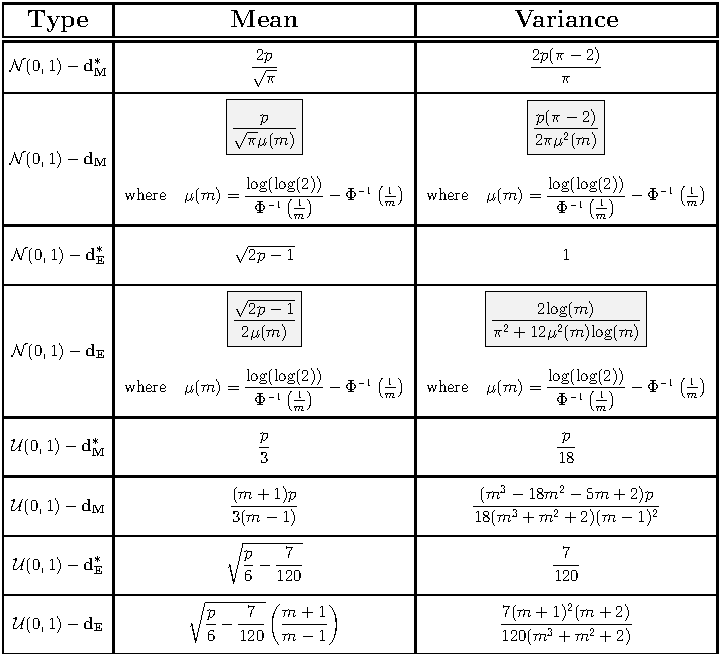
\includegraphics[width=\textwidth]{typical_data-metric_tab.pdf}
\end{table}

\begin{table}[H]
\caption{Summary of asymptotic distance distributions for rs-fMRI and GWAS data. Metrics with superscript $^*$ represent a deviation from the standard metric by attribute range normalization. The function $\Phi^{-1}(x)$ denotes the standard normal quantile function, where $x \in (0,1)$.}
\label{tab:dist_distr_bio}
\centering
% trim=left botm right top
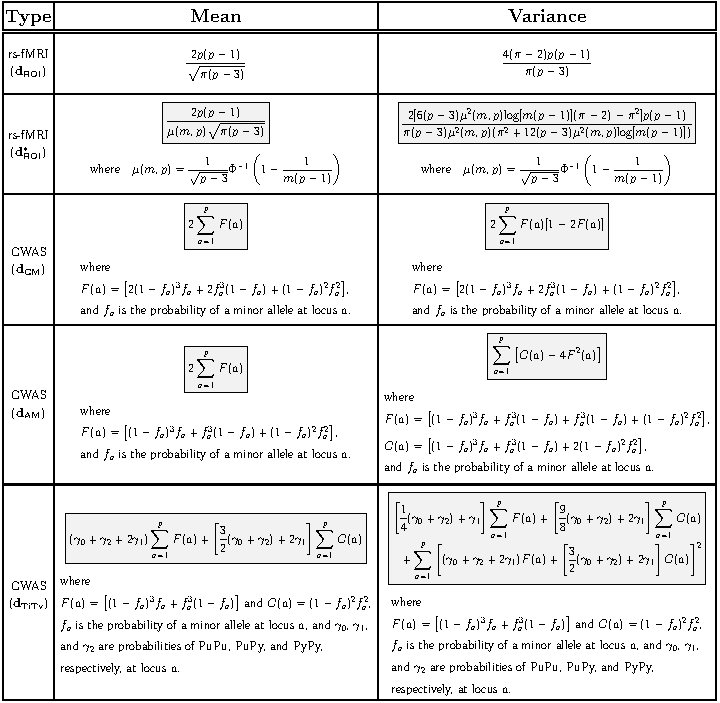
\includegraphics[width=\textwidth]{bioinformaticsy_tab.pdf}
\end{table}

\begin{table}[H]
\caption{Summary of distance distribution derivations for standard normal and standard uniform data.}
\label{tab:dist_distr_general1}
\centering
% trim=left botm right top
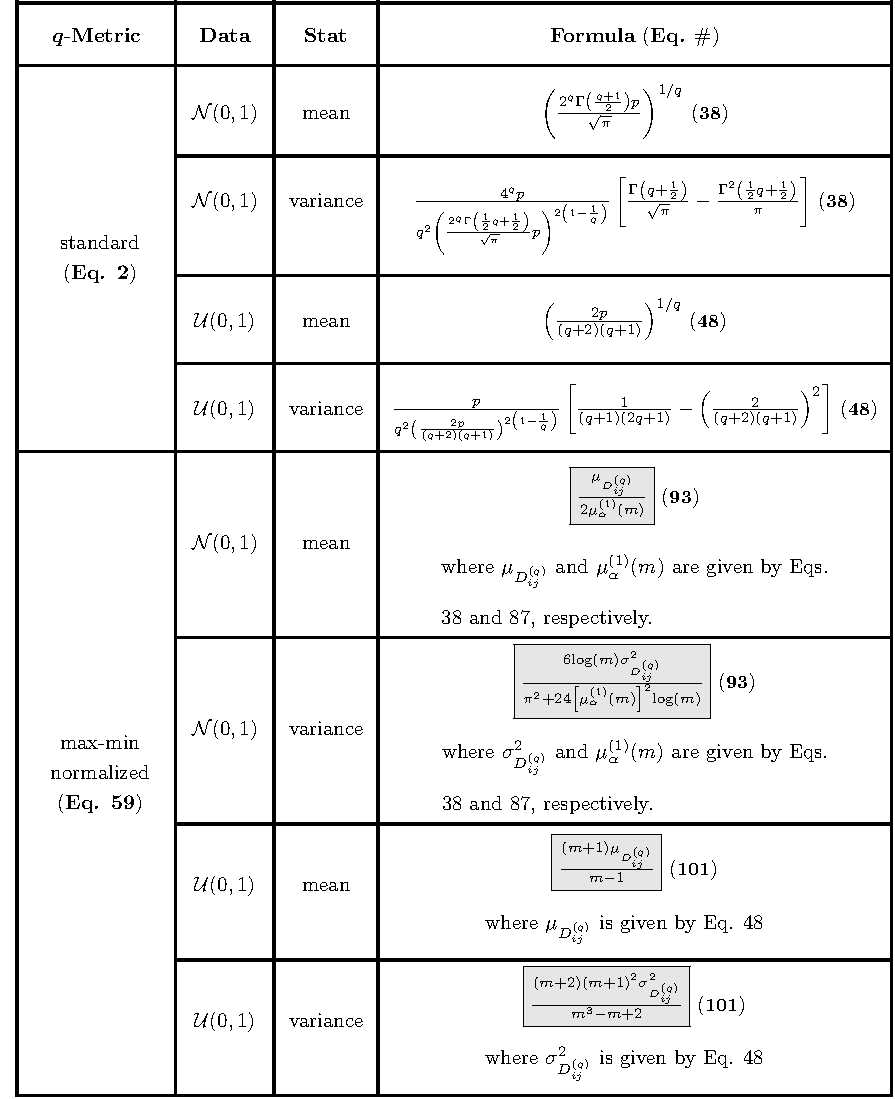
\includegraphics[clip,trim=0.27cm 0.0cm 0.0cm 0.03cm,width=\textwidth]{updated_distributions_table(5-23-2019).pdf}
\end{table}

\begin{table}[H]
\caption{Summary of distance distribution derivations for GWAS data.}
\label{tab:dist_distr_gwas}
\centering
% trim=left botm right top
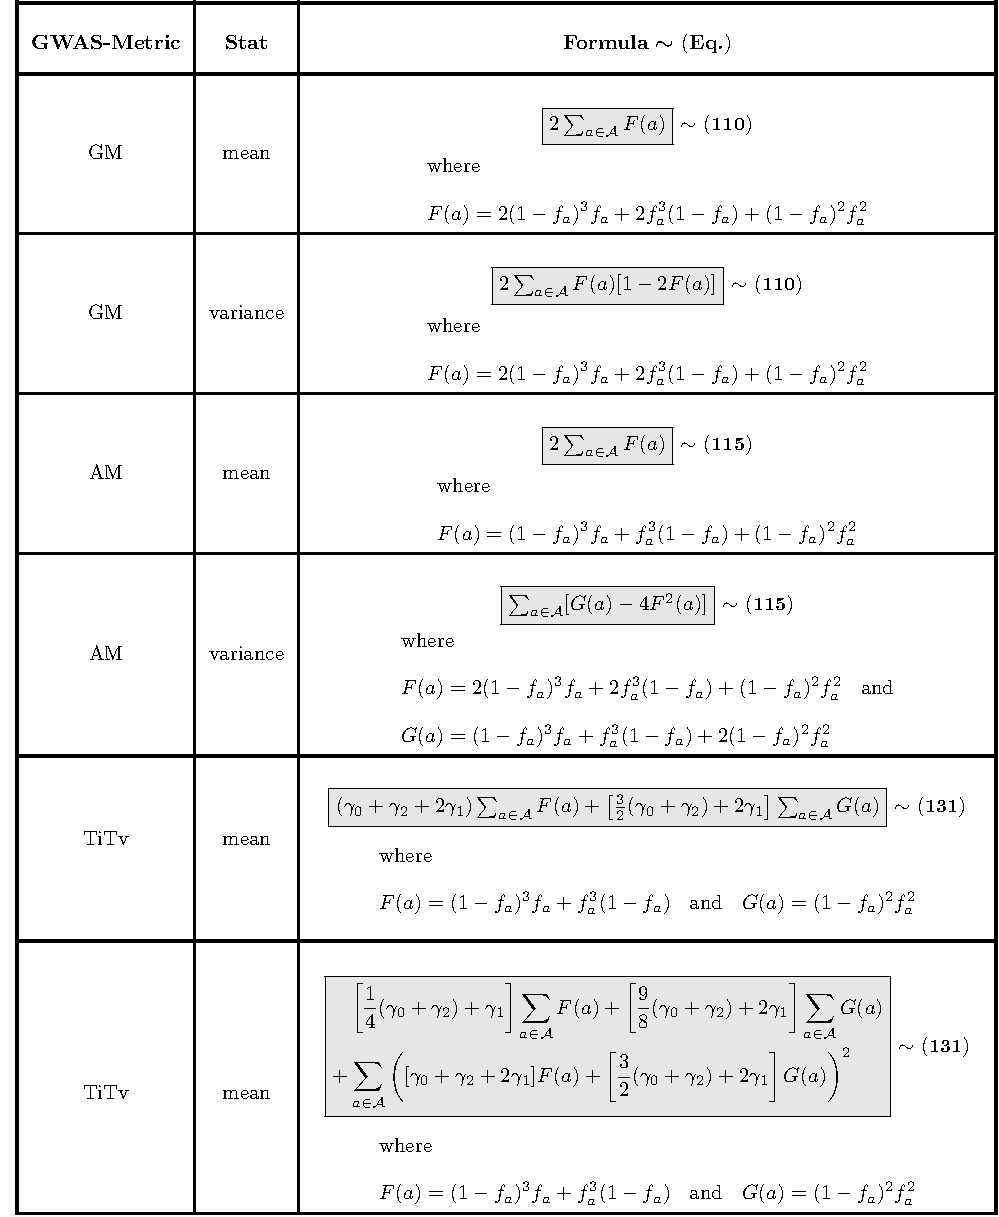
\includegraphics[clip,trim=0.27cm 0.0cm 0.0cm 0.03cm,width=\textwidth]{updated_distributions_table-gwas(5-23-2019).pdf}
\end{table}

\begin{table}[H]
\caption{Summary of distance distribution derivations for rs-fMRI data.}
\label{tab:dist_distr_rs-fMRI}
\centering
% trim=left botm right top
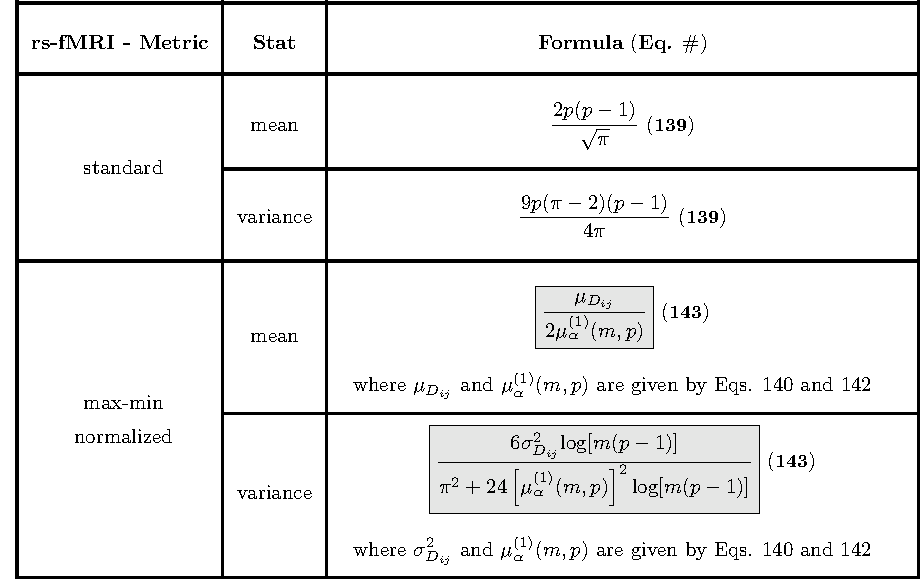
\includegraphics[clip,trim=0.27cm 0.0cm 0.0cm 0.03cm,width=\textwidth]{updated_distributions_table-rs-fMRI.pdf}
\end{table}

\section{Optimal neighborhood parameters for detecting effects}
k or $\alpha$. 
Balancing blessing and curse of dimensionality.


\section{ICA?}

Using same interaction, increase background noise genes to see degrading of A and B Relief importance because of curse of dimensionality (sparseness).  

\bibliographystyle{unsrt}
\bibliography{BoD}   % name of bib file
\end{document}
